% =====================================================================================================
% Draft: replace the prediction setting P by the re-selected setting (P2 in reports/v31_P2/).
%
% In the paper the new setting keeps the name "setting P". The first choice (theta* = 0.5, alpha_L = 0.5,
% f1 = 0.2), which this replaces, is called P$_0$ and kept as a reference where the paper reports it.
%
% How to merge into paper/main.tex (mechanical):
%   Each block below runs from "%R-BEGIN <id>" to "%R-END <id>". The lines starting with "%OLD| " give the
%   exact old text of main.tex (strip the 6-character prefix "%OLD| "; "%OLD|" alone is an empty line; join
%   with newlines). Each old text occurs exactly once in main.tex as of commit c696e7a. Replace it by the
%   lines between "%NEW-BEGIN" and "%NEW-END", verbatim.
%       python experiments/v31_P2/apply_p2_draft.py --check                  # every old text occurs once
%       python experiments/v31_P2/apply_p2_draft.py --out /tmp/main_p2.tex   # writes a merged copy
%   The script never writes main.tex itself. Labels are unchanged, so all references still resolve; three
%   figures switch to the new files paper/figures/{sim_pred_vs_n,adassp_mse_vs_eps,sweep_n}_v31p2.png.
%
% Also apply in implementation/vfr/dp.py (not edited here), the SETTINGS entry 'P':
%     'P': dict(f1=0.25, theta_star=1.5, kappa_Psi=2.0, alpha=0.05, alpha_L=0.75, alpha_U=0.0025, r1_mode='exact',
%               intervals=False),
%   and in the comment above SETTINGS: "P was re-chosen by the rule pre-registered in
%   reports/v31_P2/settings_choice_P2.md after the first choice failed on block-normalized data".
%
% Sources: reports/v31_P2/README.md and key_numbers.md (generated by experiments/v31_P2/tables_P2.py).
% =====================================================================================================

%R-BEGIN R01 Abstract: the settings, P's prediction and real-data results, the AdaSSP sentence
%OLD| We evaluate two settings of the protocol, chosen on synthetic data alone by a pre-registered rule: setting I (inference) keeps the intervals and sizes the stage-1 radius by an exact Monte Carlo quantile; setting P (prediction) gives up the intervals for a smaller ridge.
%NEW-BEGIN
We evaluate two settings of the protocol, each chosen on synthetic data alone by a pre-registered rule: setting I (inference) keeps the intervals and sizes the stage-1 radius by an exact Monte Carlo quantile; setting P (prediction) gives up the intervals for a smaller ridge, subject to its gate refusing at most $1\%$ of releases on both standardized and block-normalized synthetic features (a first choice, made on standardized features only, was refused on most block-normalized releases).
%NEW-END
%R-END R01

%R-BEGIN R02 Abstract: prediction records under P
%OLD| and prediction comes within $10\%$ of non-private test error at $2.9$k to $38$k matched records under I and $2.0$k to $23$k under P.
%NEW-BEGIN
and prediction comes within $10\%$ of non-private test error at $2.9$k to $38$k matched records under I and $2.1$k to $26$k under P.
%NEW-END
%R-END R02

%R-BEGIN R03 Abstract: real data and AdaSSP
%OLD| On real data with each party normalizing its own block of every row, setting I comes within $10\%$ of non-private test error on protein at $8.2$k and $4.1$k matched records for $\varepsilon = 1$ and $2$, but setting P fails there: its gate refuses $82$--$100\%$ of releases on bike, elevators and protein, because block normalization makes the stage-1 noise small against the stage-2 noise. Against AdaSSP on the joined table at $\varepsilon = 1$, $\delta = 10^{-6}$, v3.1 with block normalization under setting I has higher test error on $20$ of $29$ datasets (median gap $+25\%$, against $+28\%$ at the previous setting), because its ridge is still about $2.8$ times that of AdaSSP under the same guarantee. Setting P with joint normalization, which no party can apply in the vertical setting, matches AdaSSP under the same guarantee to within about $1\%$. End-to-end runs of a full OpenFHE implementation reproduce a plaintext simulation of the mechanism under all three settings.
%NEW-BEGIN
On real data with each party normalizing its own block of every row, prediction comes within $10\%$ of non-private test error on protein at $5.0$k and $2.5$k matched records for $\varepsilon = 1$ and $2$ under setting P ($8.2$k and $4.1$k under I), and P's gate refuses at most $1\%$ of releases on bike, elevators, pol and protein. Against AdaSSP on the joined table at $\varepsilon = 1$, $\delta = 10^{-6}$, v3.1 with block normalization has higher test error on $20$ of $29$ datasets under either setting, with a median gap of $+14\%$ under P and $+25\%$ under I ($+28\%$ at the previous setting), because its ridge is still larger than that of AdaSSP under the same guarantee ($1.8$ times under P and $2.8$ times under I, with joint normalization). End-to-end runs of a full OpenFHE implementation reproduce a plaintext simulation of the mechanism under every setting evaluated.
%NEW-END
%R-END R03

%R-BEGIN R04 Contributions: pre-registered rules
%OLD| under two named settings of the protocol chosen on synthetic data by a pre-registered rule: one for inference and one for prediction
%NEW-BEGIN
under two named settings of the protocol chosen on synthetic data by pre-registered rules: one for inference and one for prediction
%NEW-END
%R-END R04

%R-BEGIN R05 Section 9 (stage 2): the gate when theta* is small
%OLD| For $\vartheta^\star < 1$, as in the prediction setting P of Section~\ref{sec:params}, there is no such bound. With $\Psi = \bI$ the ridge sets $\lambda_{\min}(\hat\bG_1 + \lambda\bI) = g^\star + r_1$, so the gate passes iff
%OLD| \[
%OLD|   r_1 + \bigl[\lambda_{\min}(\hat\bG_2) - \lambda_{\min}(\hat\bG_1)\bigr] \ge (1 - \vartheta^\star)\, 2\sigma_2\sqrt p .
%OLD| \]
%OLD| The bracket is the difference of the downward shifts that the two noise levels cause in $\lambda_{\min}$; on average it is negative when $\sigma_2 > \sigma_1$. A setting with $\vartheta^\star < 1$ therefore passes only when $r_1$ is large against $\sigma_2\sqrt p$, which depends on $\Delta_G/\Delta$ and $f_1$ through~\eqref{eq:sigmas}. Section~\ref{sec:eval:sweep} shows that this fails on block-normalized real data.
%NEW-BEGIN
For $\vartheta^\star \le 2$, as in the prediction setting P of Section~\ref{sec:params} ($\vartheta^\star = 1.5$), there is no such bound. With $\Psi = \bI$ the ridge sets $\lambda_{\min}(\hat\bG_1 + \lambda\bI) = g^\star + r_1$, so the gate passes iff
\[
  r_1 + \bigl[\lambda_{\min}(\hat\bG_2) - \lambda_{\min}(\hat\bG_1)\bigr] \ge (1 - \vartheta^\star)\, 2\sigma_2\sqrt p .
\]
The bracket is the difference of the downward shifts that the two noise levels cause in $\lambda_{\min}$; on average it is negative when $\sigma_2 > \sigma_1$. With $\vartheta^\star < 1$ the right side is positive, so the gate passes only when $r_1$ is large against $\sigma_2\sqrt p$, which depends on $\Delta_G/\Delta$ and $f_1$ through~\eqref{eq:sigmas}. Block normalization makes $\Delta_G$ small against $\Delta$, and a first choice of the prediction setting with $\vartheta^\star = 0.5$ was refused on most block-normalized releases (Sections~\ref{sec:eval:adassp} and~\ref{sec:eval:sweep}). With $\vartheta^\star > 1$ the right side is negative: at $\vartheta^\star = 1.5$ the gate refuses only if the stage-2 noise lowers $\lambda_{\min}$ by more than $r_1 + \sigma_2\sqrt p$ beyond what the stage-1 noise did. Setting P was chosen under an explicit bound on the refusal rate. It refuses at most $1\%$ of releases in every simulated cell, including $\sigma_1 = 0.46\,\sigma_2$, and at most $7\%$ on any of 29 real datasets (Sections~\ref{sec:eval:sim} and~\ref{sec:eval:adassp}).
%NEW-END
%R-END R05

%R-BEGIN R06 Section 9.5: closed form of n_off under P
%OLD| and $(3.7\,\Delta + 11.0\,\Delta_G)/(\ell\sqrt{2\rho_{\mathrm{run}}})$ at setting P ($\vartheta^\star = 0.5$, $f_1 = 0.2$, $q_{0.5} = 4.94$)
%NEW-BEGIN
and $(11.5\,\Delta + 8.9\,\Delta_G)/(\ell\sqrt{2\rho_{\mathrm{run}}})$ at setting P ($\vartheta^\star = 1.5$, $f_1 = 0.25$, $q_{0.25} = 4.44$)
%NEW-END
%R-END R06

%R-BEGIN R07 Section 9.5: the transition under P
%OLD|   \item Setting P: the transition comes later. No release is off at $n_{\mathrm{off}}$, $4$--$10\%$ are off at $1.2\,n_{\mathrm{off}}$ and $56$--$70\%$ at $1.4\,n_{\mathrm{off}}$. P's radius is smaller ($q_{0.5} = 4.94$), so the downward bias of $\lambda_{\min}(\hat\bG_1)$, which the formula ignores, is a larger share of $g^\star + r_1$.
%NEW-BEGIN
  \item Setting P: the transition is wider. At most $1\%$ of releases are off at $n_{\mathrm{off}}$, $46$--$63\%$ at $1.2\,n_{\mathrm{off}}$ and $98$--$99\%$ at $1.4\,n_{\mathrm{off}}$. Its $g^\star + r_1$ is about $0.6$ times that of setting I in units of $\sigma_2$ (smaller $\vartheta^\star$, radius $q_{0.25} = 4.44$), so the downward bias of $\lambda_{\min}(\hat\bG_1)$, which the formula ignores, is a larger share of it. The first choice P$_0$ ($\vartheta^\star = 0.5$, Section~\ref{sec:params}) switched off later still: no release off at $n_{\mathrm{off}}$ and $56$--$70\%$ at $1.4\,n_{\mathrm{off}}$.
%NEW-END
%R-END R07

%R-BEGIN R08 Table tab:noff_sim: the P column
%OLD|     0.5 & 1737 & 1119 & 18{,}562 & 12{,}878 & 52{,}531 & 31{,}014 & 81{,}208 & 22{,}032 \\
%OLD|     1 & 892 & 575 & 9{,}538 & 6{,}617 & 26{,}993 & 15{,}937 & 41{,}729 & 11{,}321 \\
%OLD|     2 & 461 & 297 & 4{,}927 & 3{,}419 & 13{,}945 & 8{,}233 & 21{,}557 & 5{,}848 \\
%OLD|     4 & 240 & 155 & 2{,}569 & 1{,}783 & 7{,}272 & 4{,}293 & 11{,}241 & 3{,}050 \\
%OLD|     8 & 128 & 82 & 1{,}364 & 946 & 3{,}860 & 2{,}279 & 5{,}967 & 1{,}619 \\
%NEW-BEGIN
    0.5 & 1737 & 1119 & 18{,}562 & 12{,}878 & 52{,}531 & 31{,}014 & 81{,}208 & 31{,}498 \\
    1 & 892 & 575 & 9{,}538 & 6{,}617 & 26{,}993 & 15{,}937 & 41{,}729 & 16{,}185 \\
    2 & 461 & 297 & 4{,}927 & 3{,}419 & 13{,}945 & 8{,}233 & 21{,}557 & 8{,}361 \\
    4 & 240 & 155 & 2{,}569 & 1{,}783 & 7{,}272 & 4{,}293 & 11{,}241 & 4{,}360 \\
    8 & 128 & 82 & 1{,}364 & 946 & 3{,}860 & 2{,}279 & 5{,}967 & 2{,}314 \\
%NEW-END
%R-END R08

%R-BEGIN R09 Table tab:noff_levers: the setting-P row
%OLD|     \textbf{Setting P}: $\vartheta^\star = 0.5$, $\alpha_L = 0.5$, $f_1 = 0.2$, exact radius & 11.3k ($-73\%$) & no interval guarantee; the ridge switches off only near $1.4\,n_{\mathrm{off}}$; the gate refuses most releases where $\Delta_G \ll \Delta$ (Section~\ref{sec:eval:sweep}) \\
%NEW-BEGIN
    \textbf{Setting P}: $\vartheta^\star = 1.5$, $\alpha_L = 0.75$, $f_1 = 0.25$, exact radius & 16.2k ($-61\%$) & no interval guarantee; the ridge is off with high probability only from about $1.4\,n_{\mathrm{off}}$; a smaller $\vartheta^\star$ (P$_0$: $0.5$, 11.3k) is refused by the gate where $\Delta_G \ll \Delta$ (Section~\ref{sec:eval:sweep}) \\
%NEW-END
%R-END R09

%R-BEGIN R10 Check item on the switch-off factor
%OLD| or keep the empirical factors: 1.2 under setting I and the previous setting, about 1.5 under setting P.}
%NEW-BEGIN
or keep the empirical factors: 1.2 under setting I and the previous setting, about 1.4 under setting P.}
%NEW-END
%R-END R10

%R-BEGIN R11 Section 12: the setting-P bullet
%OLD|   \item \textbf{Setting P (prediction)} is tuned for test error only. It uses the exact-quantile radius, $\vartheta^\star = 0.5$, $\alpha_L = 0.5$, $\kappa_\Psi = 2$ and $f_1 = 0.2$. Since $\vartheta^\star < 1$ and $\alpha_L > \alpha$, the statistical results of Section~\ref{sec:stats} do not apply to it, and $\Rp$ reports the estimate without intervals. The interval guarantee holds only under setting I.
%NEW-BEGIN
  \item \textbf{Setting P (prediction)} is tuned for test error only. It uses the exact-quantile radius, $\vartheta^\star = 1.5$, $\alpha_L = 0.75$, $\kappa_\Psi = 2$ and $f_1 = 0.25$. Its intervals are off and $\alpha_L > \alpha$, so the statistical results of Section~\ref{sec:stats} do not apply to it, and $\Rp$ reports the estimate without intervals. The interval guarantee holds only under setting I. P replaces a first choice, P$_0$ ($\vartheta^\star = 0.5$, $\alpha_L = 0.5$, $f_1 = 0.2$), whose gate refused most releases on block-normalized real data. P$_0$'s results are kept for reference.
%NEW-END
%R-END R11

%R-BEGIN R12 Section 12: how P was chosen
%OLD|   \item P takes the candidate in $\vartheta^\star \in \{0.5, 1, 1.5, 2.5\} \times \alpha_L \in \{0.0025, 0.25, 0.5\} \times f_1 \in \{0.1, 0.2, 0.35\}$ that minimizes the mean ratio of test MSE to that of non-private least squares on the same cohorts, with $\btheta = 0$ for a refused release. $(0.5, 0.5, 0.2)$ wins. It lies on the edge of the grid in $\vartheta^\star$ and $\alpha_L$, and as pre-registered the grid was not extended. The five best candidates are within $0.5\%$ of each other, and no candidate's gate refused more than $2\%$ of releases in any cell on the population (the chosen one refused none).
%NEW-BEGIN
  \item P$_0$, the first choice of P, took the candidate in $\vartheta^\star \in \{0.5, 1, 1.5, 2.5\} \times \alpha_L \in \{0.0025, 0.25, 0.5\} \times f_1 \in \{0.1, 0.2, 0.35\}$ that minimized the mean ratio of test MSE to that of non-private least squares on the same cohorts, with $\btheta = 0$ for a refused release. $(0.5, 0.5, 0.2)$ won. It lay on the edge of the grid in $\vartheta^\star$ and $\alpha_L$, and as pre-registered the grid was not extended. No candidate's gate refused more than $2\%$ of releases in any cell on this population. On block-normalized real data, however, P$_0$'s gate refused most releases (Section~\ref{sec:eval:adassp}).
  \item P was then re-chosen by a second rule, also written down before any run of it (\nolinkurl{reports/v31_P2/settings_choice_P2.md}). It uses two populations: the one above, and the same cohorts with each party's block of every row scaled to unit norm ($B_R^2 = 2$, $B_O = 1$, $B_y = 2.89$). At $f_1 = 0.25$ these have $\sigma_1 = 1.55\,\sigma_2$ and $0.46\,\sigma_2$. On Wang's 29 datasets block normalization gives $0.25$--$0.83$ (median $0.56$), with 8 below $0.46$. The candidates are $\vartheta^\star \in \{0.5, 0.75, 1, 1.25, 1.5, 2, 2.5\} \times \alpha_L \in \{0.0025, 0.05, 0.25, 0.5\} \times f_1 \in \{0.1, 0.2, 0.25, 0.35\}$, with the exact radius and the intervals off. P minimizes the same criterion as P$_0$, averaged over $140$ cells (both populations, five $\varepsilon$, $14$ values of $n$, $200$ cohorts each, $R^2 = 0.5$), among the candidates whose gate refuses at most $1\%$ of releases in every cell. Ties within $0.1\%$ go to the larger $\vartheta^\star$. The grid choice $(1.5, 0.5, 0.25)$ lay on the edge in $\alpha_L$, so as pre-registered $\alpha_L = 0.75$ was added once. $(1.5, 0.75, 0.25)$ wins, with a criterion of $1.241$ against $1.274$ for I and $1.286$ for P$_0$. It lies on the edge of the extended grid and, as pre-registered, was kept. The constraint binds: six candidates with $\vartheta^\star = 1.25$ do up to $0.3\%$ better but refuse $2$--$15\%$ of releases in some block-normalized cells, and no candidate with $\vartheta^\star = 0.5$ meets it. At $R^2 = 0.3$ and $0.9$ P is also first by the criterion.
%NEW-END
%R-END R12

%R-BEGIN R13 Table tab:settings: caption and body with P and P0
%OLD| \caption{The evaluation settings. Only the statistical parameters differ. $\sigma_1$, $\sigma_2$ and $n_{\mathrm{off}}$ for the simulation population at $\varepsilon = 1$, $\delta = 10^{-9}$.}
%OLD| \label{tab:settings}
%OLD| \begin{tabular}{@{}llll@{}}
%OLD| \toprule
%OLD|  & previous (reference) & I (inference) & P (prediction) \\
%OLD| \midrule
%OLD| radius $r_1$ & union bound & exact quantile & exact quantile \\
%OLD| $r_1/\sigma_1$ at $p = 11$ & $11.53$ & $7.42$ & $4.94$ \\
%OLD| $f_1$ & $0.1$ & $0.25$ & $0.2$ \\
%OLD| $\vartheta^\star$ & $2.5$ & $2.5$ & $0.5$ \\
%OLD| $\kappa_\Psi$ & $2$ & $2$ & $2$ \\
%OLD| $\alpha_L$, $\alpha_U$ & $0.0025$, $0.0025$ & $0.0025$, $0.0025$ & $0.5$, unused \\
%OLD| intervals & yes & yes & no \\
%OLD| $\sigma_1$, $\sigma_2$ & $1411$, $525$ & $892$, $575$ & $998$, $557$ \\
%OLD| $n_{\mathrm{off}}$ & $41.7$k & $27.0$k & $11.3$k \\
%OLD| used in & Sections~\ref{sec:eval:crypto}--\ref{sec:eval:e2e} & Sections~\ref{sec:eval:sim}--\ref{sec:eval:lessons} & Sections~\ref{sec:eval:sim}, \ref{sec:eval:adassp}--\ref{sec:eval:lessons} \\
%NEW-BEGIN
\caption{The evaluation settings. Only the statistical parameters differ. $\sigma_1$, $\sigma_2$ and $n_{\mathrm{off}}$ for the simulation population at $\varepsilon = 1$, $\delta = 10^{-9}$. P$_0$ is the first choice of P, replaced because its gate refused most releases on block-normalized data.}
\label{tab:settings}
\setlength{\tabcolsep}{4pt}
\begin{tabular}{@{}lllll@{}}
\toprule
 & previous (reference) & I (inference) & P (prediction) & P$_0$ (replaced) \\
\midrule
radius $r_1$ & union bound & exact quantile & exact quantile & exact quantile \\
$r_1/\sigma_1$ at $p = 11$ & $11.53$ & $7.42$ & $4.44$ & $4.94$ \\
$f_1$ & $0.1$ & $0.25$ & $0.25$ & $0.2$ \\
$\vartheta^\star$ & $2.5$ & $2.5$ & $1.5$ & $0.5$ \\
$\kappa_\Psi$ & $2$ & $2$ & $2$ & $2$ \\
$\alpha_L$, $\alpha_U$ & $0.0025$, $0.0025$ & $0.0025$, $0.0025$ & $0.75$, unused & $0.5$, unused \\
intervals & yes & yes & no & no \\
$\sigma_1$, $\sigma_2$ & $1411$, $525$ & $892$, $575$ & $892$, $575$ & $998$, $557$ \\
$n_{\mathrm{off}}$ & $41.7$k & $27.0$k & $16.2$k & $11.3$k \\
used in & Sections~\ref{sec:eval:crypto}--\ref{sec:eval:e2e} & Sections~\ref{sec:eval:sim}--\ref{sec:eval:lessons} & Sections~\ref{sec:eval:sim}, \ref{sec:eval:adassp}--\ref{sec:eval:lessons} & as P, for reference \\
%NEW-END
%R-END R13

%R-BEGIN R14 Check item on P's grid edge
%OLD| \tocheck{Setting P's choice lies on the edge of its grid (theta-star = 0.5, alpha-L = 0.5), and at R-squared = 0.9 a larger f-1 (0.35) was better on the population. Any re-selection of a prediction setting should extend the grid in theta-star and alpha-L and include populations of different signal strength.}
%NEW-BEGIN
\tocheck{Setting P lies on the edge of the extended grid in alpha-L (0.75, so the radius is the 25 percent quantile), and its refusal constraint binds (theta-star = 1.25 would be up to 0.3 percent better on the selection populations). The selection covered sigma-1/sigma-2 down to 0.46 at f-1 = 0.25; eight of Wang's 29 datasets lie below it (solar at 0.25, where P's gate refused up to 7 percent of releases at eps = 1). Decide whether the prediction setting should depend on the noise ratio, which is public before any release.}
%NEW-END
%R-END R14

%R-BEGIN R15 Table tab:params: f1 row
%OLD| & I: $0.25$; P: $0.2$ (previous: $0.1$) \\
%NEW-BEGIN
& I and P: $0.25$ (previous: $0.1$) \\
%NEW-END
%R-END R15

%R-BEGIN R16 Table tab:params: theta* row
%OLD| coverage is asymptotic in $\vartheta^\star$ (Remark~\ref{rem:firstorder}) & I: $2.5$; P: $0.5$ \\
%NEW-BEGIN
coverage is asymptotic in $\vartheta^\star$ (Remark~\ref{rem:firstorder}) & I: $2.5$; P: $1.5$ \\
%NEW-END
%R-END R16

%R-BEGIN R17 Table tab:params: alpha row
%OLD| P: intervals off, $\alpha_L = 0.5$ \\
%NEW-BEGIN
P: intervals off, $\alpha_L = 0.75$ \\
%NEW-END
%R-END R17

%R-BEGIN R18 Section 12, derived quantities: noise under P
%OLD| ; at setting P ($f_1 = 0.2$) $\sigma_1 = 997.8$ and $\sigma_2 = 556.9$.
%NEW-BEGIN
; setting P has the same $f_1$ and so the same noise (P$_0$, with $f_1 = 0.2$: $\sigma_1 = 997.8$ and $\sigma_2 = 556.9$).
%NEW-END
%R-END R18

%R-BEGIN R19 Section 13.2: sigma_2 under P
%OLD| and $1.061$ times at setting P ($f_1 = 0.2$);
%NEW-BEGIN
and at setting P, which has the same $f_1$;
%NEW-END
%R-END R19

%R-BEGIN R20 Section 13.5 setup: what is added for P
%OLD| and adds setting P for prediction.
%NEW-BEGIN
and adds setting P for prediction, with its first choice P$_0$ for reference. For P it also uses a block-normalized version of the population, on the same cohorts and noise draws.
%NEW-END
%R-END R20

%R-BEGIN R21 Section 13.5: switch-off under P
%OLD|   \item Under setting P the switch-off comes later relative to its own $n_{\mathrm{off}}$ (Section~\ref{sec:stats:noff}): no release is off at $n_{\mathrm{off}}$, $4$--$10\%$ at $1.2\,n_{\mathrm{off}}$ and $56$--$70\%$ at $1.4\,n_{\mathrm{off}}$, and at $0.8\,n_{\mathrm{off}}$ the rule chooses $3.0$--$3.4$ times the linear prediction.
%NEW-BEGIN
  \item Under setting P the switch-off is wider relative to its own $n_{\mathrm{off}}$ (Section~\ref{sec:stats:noff}): at most $1\%$ of releases are off at $n_{\mathrm{off}}$, $46$--$63\%$ at $1.2\,n_{\mathrm{off}}$ and $98$--$99\%$ at $1.4\,n_{\mathrm{off}}$, and at $0.8\,n_{\mathrm{off}}$ the rule chooses $2.0$--$2.3$ times the linear prediction. Under P$_0$ only $56$--$70\%$ were off at $1.4\,n_{\mathrm{off}}$, and the factor at $0.8\,n_{\mathrm{off}}$ was $3.0$--$3.4$.
%NEW-END
%R-END R21

%R-BEGIN R22 Section 13.5: validity ratio held under P
%OLD| Setting P holds it at $2.9$--$3.0$.
%NEW-BEGIN
Setting P holds it at $3.4$--$3.5$, and at $2.0$ on the block-normalized population (I: $3.2$; P$_0$: $2.9$--$3.0$ and $1.1$--$1.2$).
%NEW-END
%R-END R22

%R-BEGIN R23 Section 13.5: prediction paragraph
%OLD| \paragraph{Prediction recovers first, and fastest under setting P.} On a held-out sample of the population (clipped design, unclipped $y$), setting I brings the test MSE within $10\%$ of that of non-private least squares at $n \approx 38$k, $20$k, $10$k, $5.3$k and $2.9$k for $\varepsilon = 0.5$ to $8$ ($0.72$--$0.76\,n_{\mathrm{off}}$, while the ridge is still on). The previous setting needed $58$k, $30$k, $15$k, $8.0$k and $4.2$k. Setting P, which was chosen for this, needs $23$k, $12$k, $6.2$k, $3.6$k and $2.0$k (Figure~\ref{fig:sim_pred_v31s}): $1.5$--$1.7$ times fewer records than I and $2.2$--$2.5$ times fewer than the previous setting. Within $1\%$ the settings are closer: $68$k to $4.9$k for P, $72$k to $5.0$k for I, and $91$k to $7.0$k for the previous setting. P's advantage over I shrinks with a stronger signal. At $R^2 = 0.9$ P needs $1.06$--$1.25$ times fewer records than I ($\varepsilon = 1$: $27$k against $32$k); at $R^2 = 0.3$ it needs $1.5$--$1.7$ times fewer. The gate refused no release under either setting, at any $R^2$ and $n$. Under setting I, twice-the-floor accuracy on the coefficients needs $2.8$, $5.0$ and $8.8$ times as many records as prediction within $10\%$, for $\varepsilon = 8$, $4$ and $2$.
%NEW-BEGIN
\paragraph{Prediction recovers first, and fastest under setting P.} On a held-out sample of the population (clipped design, unclipped $y$), setting I brings the test MSE within $10\%$ of that of non-private least squares at $n \approx 38$k, $20$k, $10$k, $5.3$k and $2.9$k for $\varepsilon = 0.5$ to $8$ ($0.72$--$0.76\,n_{\mathrm{off}}$, while the ridge is still on). The previous setting needed $58$k, $30$k, $15$k, $8.0$k and $4.2$k. Setting P, which was chosen for this, needs $26$k, $14$k, $7.1$k, $4.0$k and $2.1$k (Figure~\ref{fig:sim_pred_v31s}). That is $1.3$--$1.5$ times fewer records than I and $2.0$--$2.2$ times fewer than the previous setting. On this population the first choice P$_0$ needed $5$--$13\%$ fewer records than P ($23$k, $12$k, $6.2$k, $3.6$k and $2.0$k). Within $1\%$ the settings are close: $70$k to $5.0$k for P, $72$k to $5.0$k for I, and $91$k to $7.0$k for the previous setting. P's advantage over I shrinks with a stronger signal. At $R^2 = 0.9$ P needs $1.04$--$1.20$ times fewer records than I ($\varepsilon = 1$: $28$k against $32$k); at $R^2 = 0.3$ it needs $1.3$--$1.4$ times fewer. On this population the gate refused no release under I or P, at any $R^2$ and $n$. Under setting I, twice-the-floor accuracy on the coefficients needs $2.8$, $5.0$ and $8.8$ times as many records as prediction within $10\%$, for $\varepsilon = 8$, $4$ and $2$.

\paragraph{The block-normalized population.} The bottom row of Figure~\ref{fig:sim_pred_v31s} uses the same cohorts with each party's block of every row scaled to unit norm ($B_R^2 = 2$, $B_O = 1$, $B_y = 2.89$; $\Delta = 10.2$, $\Delta_G = 2.83$, $\ell = 0.105$). There $\sigma_1 = 0.46\,\sigma_2$ at $f_1 = 0.25$, against $1.55\,\sigma_2$ above, and P's $n_{\mathrm{off}}$ is $16$k to $1.2$k for $\varepsilon = 0.5$ to $8$.
\begin{itemize}[noitemsep]
  \item Setting P comes within $10\%$ at $9.4$k, $4.8$k, $2.5$k, $1.5$k and $729$ matched records, against $15$k, $7.5$k, $4.0$k, $2.1$k and $1.1$k under I ($1.4$--$1.6$ times fewer).
  \item Its gate refused at most $1\%$ of releases in any cell, $0.06\%$ on average, and also at most $1\%$ at $R^2 = 0.3$ and $0.9$.
  \item P$_0$'s gate refused $98$--$100\%$ of releases wherever its ridge was on, so its test MSE stays near that of predicting the mean until the ridge switches off.
\end{itemize}
%NEW-END
%R-END R23

%R-BEGIN R24 Figure fig:sim_pred_v31s: new file and caption
%OLD|   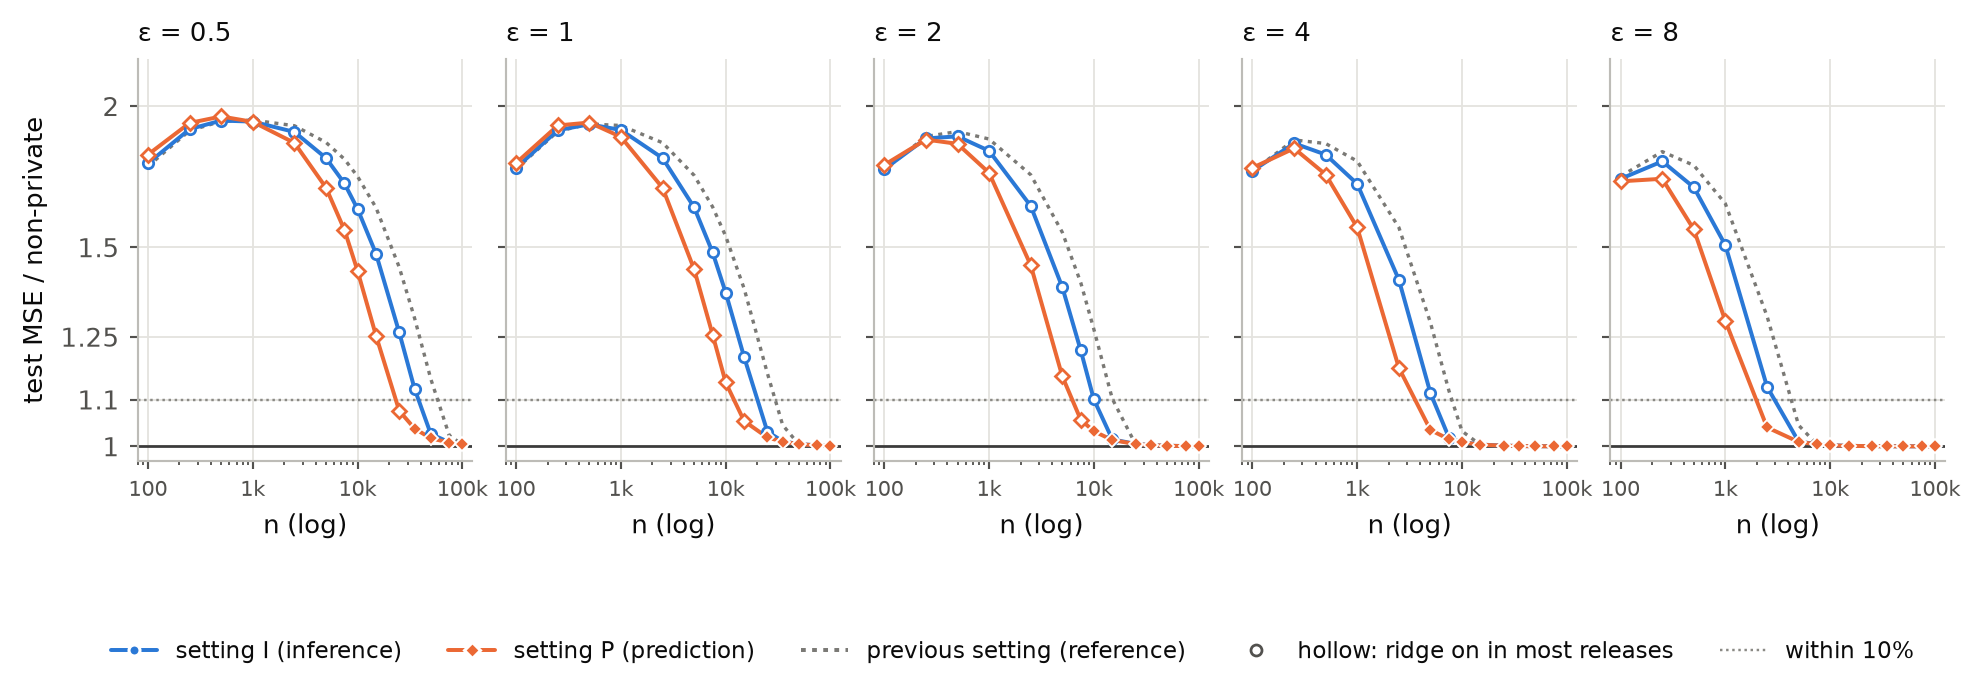
\includegraphics[width=\textwidth]{figures/sim_pred_vs_n_v31s.png}
%OLD|   \caption{Test MSE on the population divided by that of non-private least squares on the same cohort, against $n$, $\delta = 10^{-9}$, $R^2 = 0.5$; mean over 200 cohorts, a refused release counted as $\btheta = 0$ (there were none). Blue: setting I. Orange: setting P. Grey dotted: the previous setting. Hollow markers: the stage-1 ridge is on in most releases. Dotted horizontal: within $10\%$.}
%NEW-BEGIN
  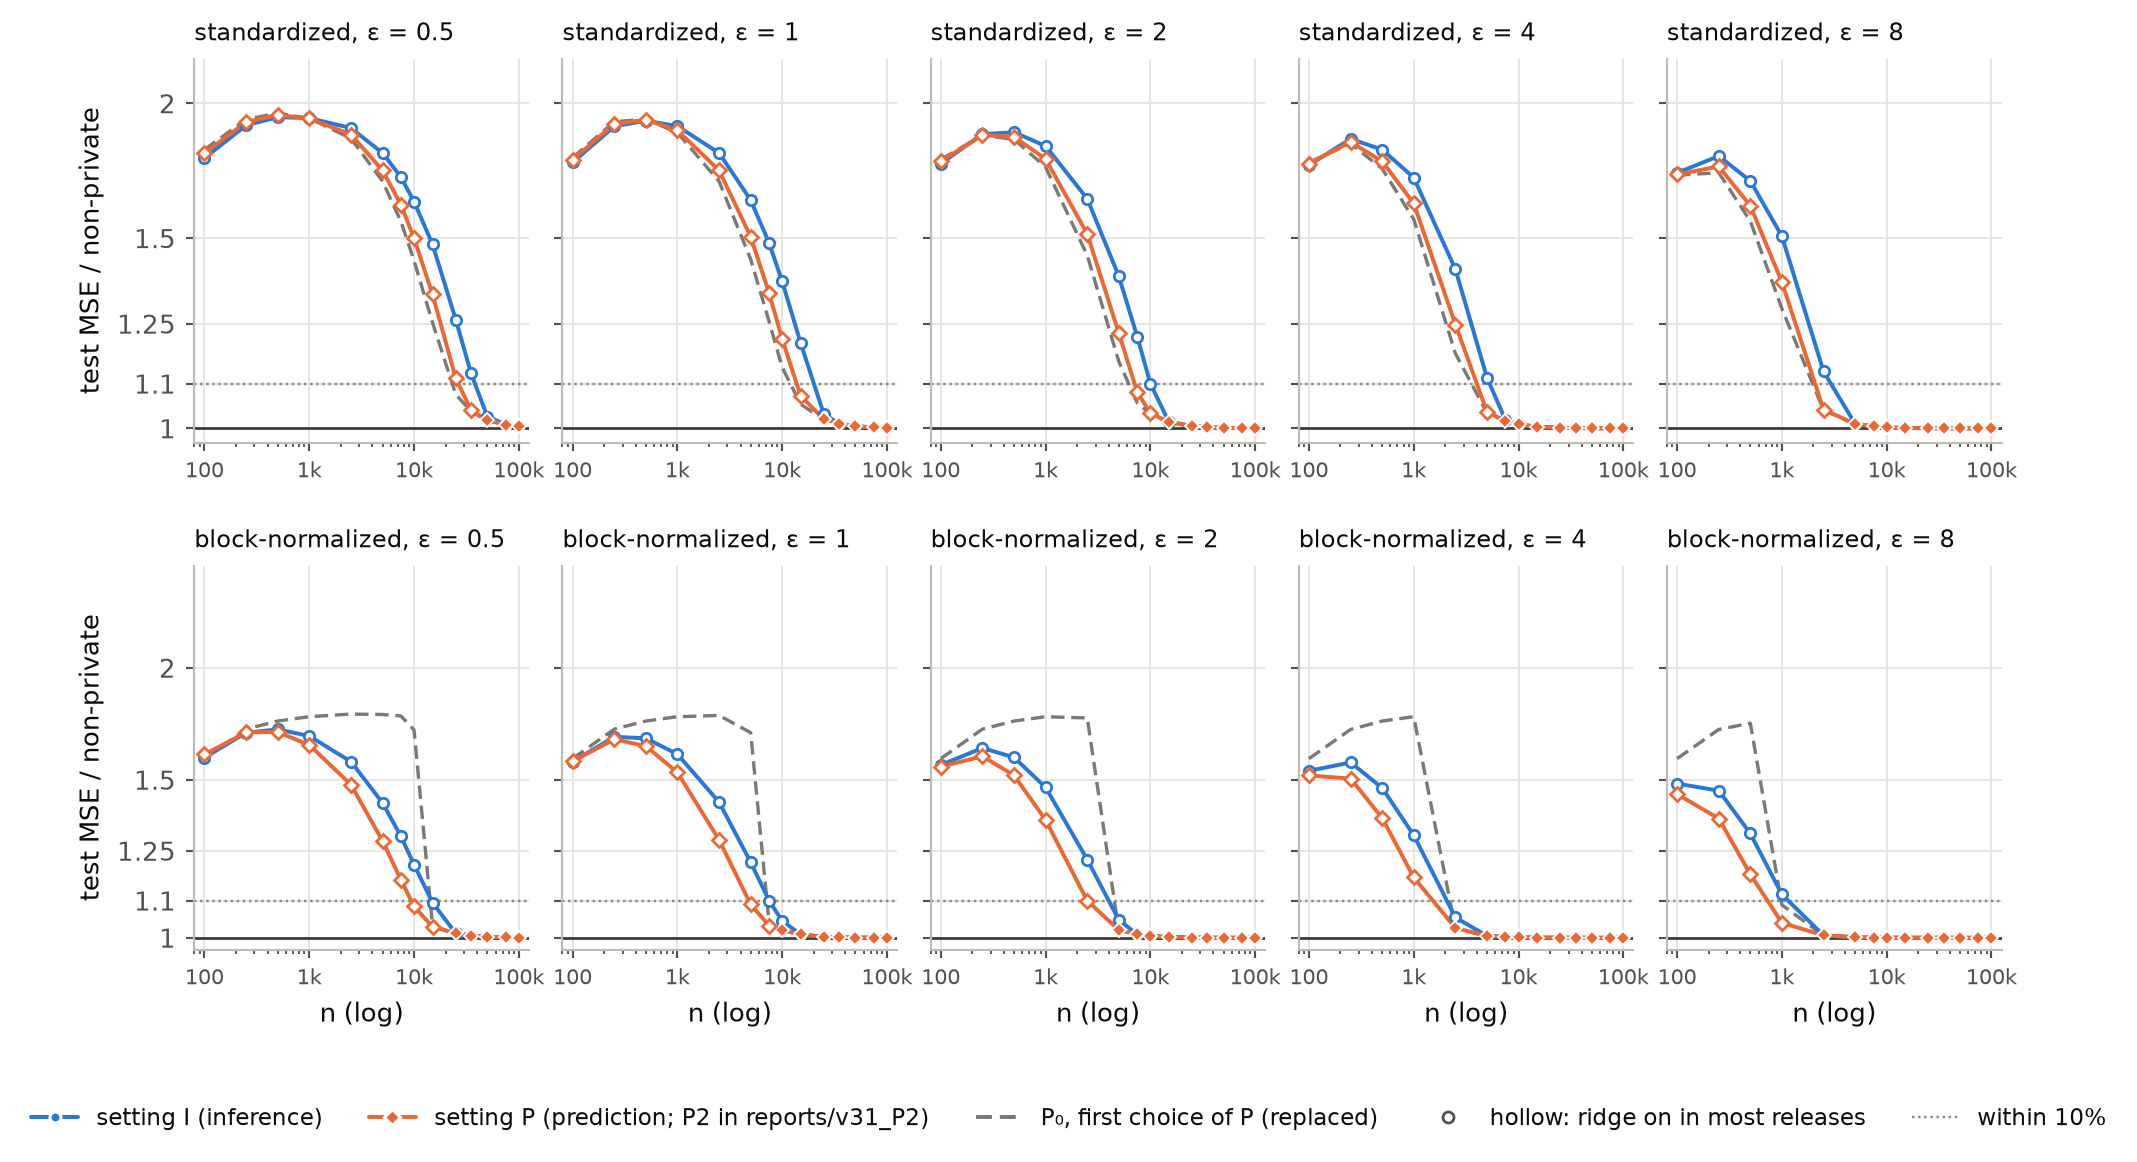
\includegraphics[width=\textwidth]{figures/sim_pred_vs_n_v31p2.png}
  \caption{Test MSE on the population divided by that of non-private least squares on the same cohort, against $n$, $\delta = 10^{-9}$, $R^2 = 0.5$. Top row: the standardized population. Bottom row: the same cohorts with block-normalized features. Mean over 200 cohorts, a refused release counted as $\btheta = 0$. Blue: setting I. Orange: setting P. Grey dashed: P$_0$, the first choice of P, whose gate refuses the block-normalized releases while its ridge is on. Hollow markers: the stage-1 ridge is on in most releases. Dotted horizontal: within $10\%$.}
%NEW-END
%R-END R24

%R-BEGIN R25 Section 13.5: encrypted check
%OLD| \paragraph{Encrypted check of settings I and P.} We ran the full OpenFHE implementation ten times on one synthetic dataset from this population: $n = 10{,}000$ matched records in a register of $12{,}000$ rows padded to $16{,}384$, $\delta = 10^{-9}$. Five runs used setting I at $\varepsilon = 2$ and five used setting P at $\varepsilon = 1$; in both the ridge is on (the matched design's $n_{\mathrm{off}}$ is $14.1$k and $11.5$k, and P switches off only near $1.4\,n_{\mathrm{off}}$). Each run took $29$--$31$\,s. $\Rp$ read the exact radius from the cached quantile: $r_1 = 3{,}419$ under I and $4{,}929$ under P.
%OLD| \begin{itemize}[noitemsep]
%OLD|   \item The ridge chosen in every run lay inside the $95\%$ range of a plaintext simulation of the same mechanism on the same data (4{,}000 draws): $3{,}162$--$3{,}729$ against $2{,}578$--$4{,}232$ under I, and $3{,}890$--$4{,}897$ against $2{,}197$--$5{,}543$ under P. No release was refused.
%OLD|   \item Against the simulated distribution of $\tilde\btheta$ given each run's $\lambda$, $54$ of $55$ encrypted coefficients lay within $2.5$ s.d.\ under each setting (largest $2.91$ and $2.58$ s.d.). Under I the Wald interval covered $\btheta_\lambda$ for $54$ of $55$ coefficients.
%OLD|   \item The raw decrypted noise on the $510$ stage-1 and $620$ stage-2 entries, standardized by the calibrated $\sigma_1$ and $\sigma_2$, had s.d.\ $1.00$ and mean $0.00$ pooled (Kolmogorov--Smirnov $p = 0.79$ against $\mathcal N(0, 1)$), s.d.\ $0.96$--$1.08$ for each setting and stage, and no value beyond $3.3$. $\bA$ was exact.
%NEW-BEGIN
\paragraph{Encrypted check of settings I and P.} We ran the full OpenFHE implementation fifteen times on one synthetic dataset from this population: $n = 10{,}000$ matched records in a register of $12{,}000$ rows padded to $16{,}384$, $\delta = 10^{-9}$. Five runs used setting I at $\varepsilon = 2$, five used setting P at $\varepsilon = 1$, and five, made earlier, used P$_0$ at $\varepsilon = 1$. In all of them the ridge is on: the matched design's $n_{\mathrm{off}}$ is $14.1$k, $16.4$k and $11.5$k. Each run took $29$--$31$\,s. $\Rp$ read the exact radius from the cached quantile: $r_1 = 3{,}419$ under I, $3{,}964$ under P and $4{,}929$ under P$_0$.
\begin{itemize}[noitemsep]
  \item The ridge chosen in every run lay inside the $95\%$ range of a plaintext simulation of the same mechanism on the same data (4{,}000 draws): $3{,}162$--$3{,}729$ against $2{,}578$--$4{,}232$ under I, $4{,}924$--$6{,}708$ against $4{,}837$--$7{,}855$ under P, and $3{,}890$--$4{,}897$ against $2{,}197$--$5{,}543$ under P$_0$. No release was refused.
  \item Against the simulated distribution of $\tilde\btheta$ given each run's $\lambda$, $54$ of $55$ encrypted coefficients lay within $2.5$ s.d.\ under each setting (largest $2.91$, $2.59$ and $2.58$ s.d.). Under I the Wald interval covered $\btheta_\lambda$ for $54$ of $55$ coefficients.
  \item The raw decrypted noise on the $765$ stage-1 and $930$ stage-2 entries, standardized by the calibrated $\sigma_1$ and $\sigma_2$, had s.d.\ $0.99$ and mean $-0.03$ pooled (Kolmogorov--Smirnov $p = 0.46$ against $\mathcal N(0, 1)$). Its s.d.\ was $0.95$--$1.08$ for each setting and stage, and no value lay beyond $3.3$. The five runs under P alone had mean $-0.10$ (standard error $0.04$) and s.d.\ $0.97$ ($p = 0.17$). $\bA$ was exact.
%NEW-END
%R-END R25

%R-BEGIN R26 Check item on the size of the encrypted checks
%OLD| 5 runs each for settings I and P and 10 for the previous setting, at one epsilon each.
%NEW-BEGIN
5 runs each for settings I, P and P-0 and 10 for the previous setting, at one epsilon each.
%NEW-END
%R-END R26

%R-BEGIN R27 Section 13.7 setup: shared noise draws
%OLD| Settings I and P of one preprocessing share their unit noise draws.
%NEW-BEGIN
Settings I, P and P$_0$ of one preprocessing share their unit noise draws. P was run after the other two, on the same draws; rerunning I on them reproduced its test MSE to within $10^{-14}$ (relative).
%NEW-END
%R-END R27

%R-BEGIN R28 Table tab:adassp_v31: P columns
%OLD|     housing & 506 & 13 & 1.83 & 2.05 & 2.35 & 2.13 & 2.44 & 2.87 & 3.13 & 2.50 \\
%OLD|     wine & 1{,}599 & 11 & 1.75 & 1.94 & 2.21 & 1.95 & 1.87 & 2.24 & 3.02 & 1.92 \\
%OLD|     airfoil & 1{,}503 & 5 & 1.10 & 1.16 & 1.34 & 1.27 & 1.43 & 1.74 & 1.76 & 1.51 \\
%OLD|     concrete & 1{,}030 & 8 & 1.53 & 1.73 & 2.18 & 1.78 & 2.56 & 3.16 & 2.31 & 2.69 \\
%OLD|     bike & 17{,}379 & 17 & 1.04 & 1.07 & 1.22 & 1.08 & 1.38 & 3.93 & 1.47 & 1.43 \\
%OLD|     elevators & 16{,}599 & 18 & 1.57 & 1.77 & 2.26 & 1.91 & 1.13 & 1.60 & 2.68 & 1.13 \\
%OLD|     pol & 15{,}000 & 26 & 1.05 & 1.08 & 1.26 & 1.11 & 1.53 & 1.27 & 1.66 & 1.63 \\
%OLD|     kin40k & 40{,}000 & 8 & 1.00 & 1.00 & 1.00 & 1.00 & 1.00 & 1.00 & 1.00 & 1.00 \\
%OLD|     protein & 45{,}730 & 9 & 1.01 & 1.01 & 1.03 & 1.02 & 1.02 & 1.35 & 1.12 & 1.03 \\
%NEW-BEGIN
    housing & 506 & 13 & 1.83 & 2.05 & 2.35 & 2.22 & 2.44 & 2.28 & 3.13 & 2.50 \\
    wine & 1{,}599 & 11 & 1.75 & 1.94 & 2.21 & 2.06 & 1.87 & 1.73 & 3.02 & 1.92 \\
    airfoil & 1{,}503 & 5 & 1.10 & 1.16 & 1.34 & 1.19 & 1.43 & 1.27 & 1.76 & 1.51 \\
    concrete & 1{,}030 & 8 & 1.53 & 1.73 & 2.18 & 1.94 & 2.56 & 2.26 & 2.31 & 2.69 \\
    bike & 17{,}379 & 17 & 1.04 & 1.07 & 1.22 & 1.13 & 1.38 & 1.22 & 1.47 & 1.43 \\
    elevators & 16{,}599 & 18 & 1.57 & 1.77 & 2.26 & 2.07 & 1.13 & 1.10 & 2.68 & 1.13 \\
    pol & 15{,}000 & 26 & 1.05 & 1.08 & 1.26 & 1.16 & 1.53 & 1.38 & 1.66 & 1.63 \\
    kin40k & 40{,}000 & 8 & 1.00 & 1.00 & 1.00 & 1.00 & 1.00 & 1.00 & 1.00 & 1.00 \\
    protein & 45{,}730 & 9 & 1.01 & 1.01 & 1.03 & 1.02 & 1.02 & 1.01 & 1.12 & 1.03 \\
%NEW-END
%R-END R28

%R-BEGIN R29 Table tab:adassp_abs_v31: P columns
%OLD|     housing & 0.0400 & 0.0396 & \textbf{0.0732} & 0.0821 & 0.0941 & 0.0851 & 0.0966 & 0.114 & 0.0990 \\
%OLD|     wine & 0.0201 & 0.0252 & \textbf{0.0350} & 0.0390 & 0.0444 & 0.0393 & 0.0472 & 0.0565 & 0.0485 \\
%OLD|     airfoil & 0.0534 & 0.0521 & \textbf{0.0586} & 0.0622 & 0.0715 & 0.0678 & 0.0746 & 0.0906 & 0.0787 \\
%OLD|     concrete & 0.0445 & 0.0381 & \textbf{0.0681} & 0.0770 & 0.0968 & 0.0792 & 0.0977 & 0.120 & 0.103 \\
%OLD|     bike & 0.0279 & 0.0270 & \textbf{0.0290} & 0.0299 & 0.0341 & 0.0301 & 0.0372 & 0.106 & 0.0388 \\
%OLD|     elevators & 0.00872 & 0.0229 & \textbf{0.0136} & 0.0154 & 0.0197 & 0.0166 & 0.0259 & 0.0367 & 0.0260 \\
%OLD|     pol & 0.135 & 0.123 & \textbf{0.141} & 0.146 & 0.170 & 0.149 & 0.188 & 0.156 & 0.201 \\
%OLD|     kin40k & 0.0632 & 0.0632 & 0.0633 & 0.0633 & 0.0633 & 0.0633 & \textbf{0.0632} & \textbf{0.0632} & 0.0632 \\
%OLD|     protein & 0.119 & 0.121 & \textbf{0.120} & 0.120 & 0.122 & 0.121 & 0.124 & 0.163 & 0.124 \\
%NEW-BEGIN
    housing & 0.0400 & 0.0396 & \textbf{0.0732} & 0.0821 & 0.0941 & 0.0889 & 0.0966 & 0.0902 & 0.0990 \\
    wine & 0.0201 & 0.0252 & \textbf{0.0350} & 0.0390 & 0.0444 & 0.0413 & 0.0472 & 0.0438 & 0.0485 \\
    airfoil & 0.0534 & 0.0521 & \textbf{0.0586} & 0.0622 & 0.0715 & 0.0638 & 0.0746 & 0.0661 & 0.0787 \\
    concrete & 0.0445 & 0.0381 & \textbf{0.0681} & 0.0770 & 0.0968 & 0.0865 & 0.0977 & 0.0861 & 0.103 \\
    bike & 0.0279 & 0.0270 & \textbf{0.0290} & 0.0299 & 0.0341 & 0.0315 & 0.0372 & 0.0329 & 0.0388 \\
    elevators & 0.00872 & 0.0229 & \textbf{0.0136} & 0.0154 & 0.0197 & 0.0180 & 0.0259 & 0.0253 & 0.0260 \\
    pol & 0.135 & 0.123 & \textbf{0.141} & 0.146 & 0.170 & 0.157 & 0.188 & 0.170 & 0.201 \\
    kin40k & 0.0632 & 0.0632 & 0.0633 & 0.0633 & 0.0633 & 0.0633 & \textbf{0.0632} & \textbf{0.0632} & 0.0632 \\
    protein & 0.119 & 0.121 & \textbf{0.120} & 0.120 & 0.122 & 0.121 & 0.124 & 0.122 & 0.124 \\
%NEW-END
%R-END R29

%R-BEGIN R30 Table tab:verdicts_v31: rows for P and P0
%OLD|     (d) block, P vs (a) & 6 / 19 & 5 / 20 & 3 / 21 & 2 / 24 & 2 / 22 \\
%OLD|     (d) block, previous vs (a) & 5 / 19 & 5 / 19 & 4 / 21 & 3 / 23 & 1 / 21 \\
%OLD|     \midrule
%OLD|     (c) joint, I vs (a) AdaSSP, published & 7 / 19 & 5 / 23 & 4 / 23 & 1 / 21 & 0 / 22 \\
%OLD|     (c) joint, P vs (a) & 6 / 20 & 4 / 22 & 1 / 25 & 0 / 24 & 0 / 26 \\
%OLD|     (c) joint, previous vs (a) & 7 / 19 & 6 / 20 & 3 / 22 & 2 / 22 & 0 / 23 \\
%OLD|     \midrule
%OLD|     (c) joint, I vs (b) AdaSSP, matched & 8 / 15 & 6 / 18 & 6 / 20 & 5 / 19 & 2 / 20 \\
%OLD|     (c) joint, P vs (b) & 11 / 10 & 6 / 11 & 6 / 12 & 5 / 12 & 3 / 12 \\
%OLD|     (c) joint, previous vs (b) & 10 / 17 & 8 / 18 & 5 / 20 & 5 / 21 & 3 / 20 \\
%OLD|     \midrule
%OLD|     (d) block, I vs (d) block, previous & 18 / 4 & 19 / 1 & 21 / 1 & 23 / 1 & 24 / 0 \\
%OLD|     (d) block, P vs (d) block, I & 4 / 20 & 3 / 19 & 3 / 19 & 3 / 20 & 5 / 16 \\
%OLD|     (c) joint, P vs (c) joint, I & 20 / 8 & 20 / 6 & 21 / 6 & 20 / 5 & 20 / 4 \\
%NEW-BEGIN
    (d) block, P vs (a) & 6 / 19 & 5 / 20 & 5 / 18 & 2 / 20 & 3 / 15 \\
    (d) block, P$_0$ vs (a) & 6 / 19 & 5 / 20 & 3 / 21 & 2 / 24 & 2 / 22 \\
    (d) block, previous vs (a) & 5 / 19 & 5 / 19 & 4 / 21 & 3 / 23 & 1 / 21 \\
    (d) block, P vs (b) AdaSSP, matched & 9 / 16 & 5 / 19 & 6 / 18 & 5 / 14 & 9 / 15 \\
    \midrule
    (c) joint, I vs (a) AdaSSP, published & 7 / 19 & 5 / 23 & 4 / 23 & 1 / 21 & 0 / 22 \\
    (c) joint, P vs (a) & 6 / 20 & 5 / 22 & 3 / 24 & 0 / 23 & 0 / 25 \\
    (c) joint, P$_0$ vs (a) & 6 / 20 & 4 / 22 & 1 / 25 & 0 / 24 & 0 / 26 \\
    (c) joint, previous vs (a) & 7 / 19 & 6 / 20 & 3 / 22 & 2 / 22 & 0 / 23 \\
    \midrule
    (c) joint, I vs (b) AdaSSP, matched & 8 / 15 & 6 / 18 & 6 / 20 & 5 / 19 & 2 / 20 \\
    (c) joint, P vs (b) & 8 / 15 & 6 / 18 & 6 / 18 & 4 / 18 & 1 / 18 \\
    (c) joint, P$_0$ vs (b) & 11 / 10 & 6 / 11 & 6 / 12 & 5 / 12 & 3 / 12 \\
    (c) joint, previous vs (b) & 10 / 17 & 8 / 18 & 5 / 20 & 5 / 21 & 3 / 20 \\
    \midrule
    (d) block, I vs (d) block, previous & 18 / 4 & 19 / 1 & 21 / 1 & 23 / 1 & 24 / 0 \\
    (d) block, P vs (d) block, I & 18 / 2 & 21 / 1 & 23 / 1 & 24 / 1 & 23 / 0 \\
    (d) block, P vs (d) block, P$_0$ & 20 / 5 & 19 / 4 & 19 / 4 & 20 / 3 & 18 / 4 \\
    (c) joint, P vs (c) joint, I & 18 / 7 & 19 / 6 & 21 / 5 & 20 / 3 & 20 / 2 \\
    (c) joint, P vs (c) joint, P$_0$ & 7 / 18 & 7 / 20 & 8 / 19 & 6 / 20 & 7 / 19 \\
%NEW-END
%R-END R30

%R-BEGIN R31 Figure fig:adassp_v31: new file and caption
%OLD|   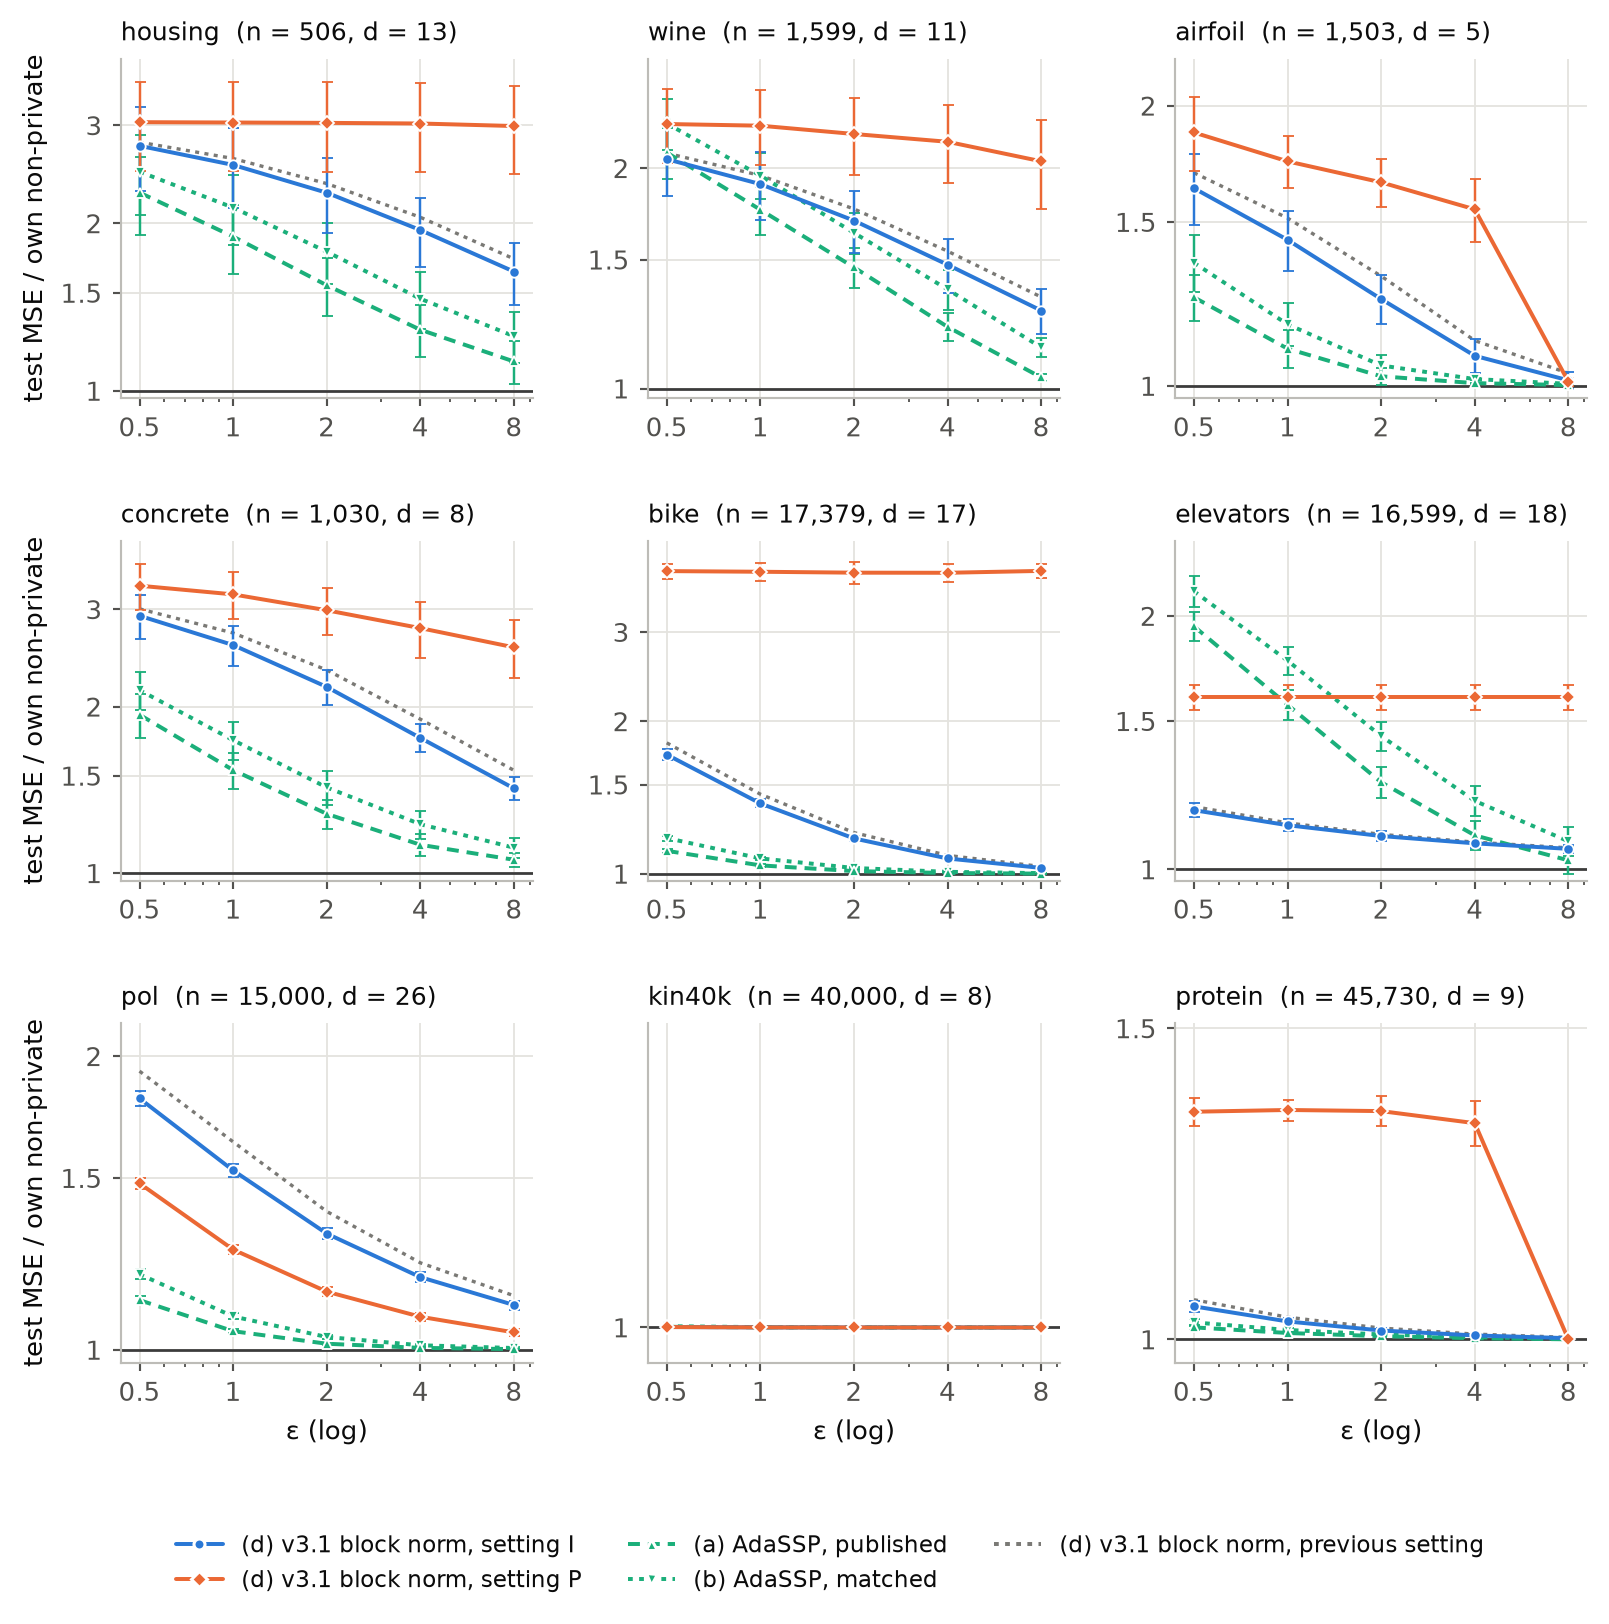
\includegraphics[width=\textwidth]{figures/adassp_mse_vs_eps_v31s.png}
%OLD|   \caption{Test MSE divided by each arm's own non-private test MSE against $\varepsilon$, $\delta = 10^{-6}$, on nine of the datasets. Blue: v3.1 with block unit norm, setting I. Orange: the same, setting P. Aqua: AdaSSP, published (dashed) and matched (dotted). Grey dotted: v3.1 with block unit norm at the previous setting, from its earlier run. Points: mean over 10 folds and 50 noise draws. Error bars: 95\% CI of the mean ($t$ over folds).}
%NEW-BEGIN
  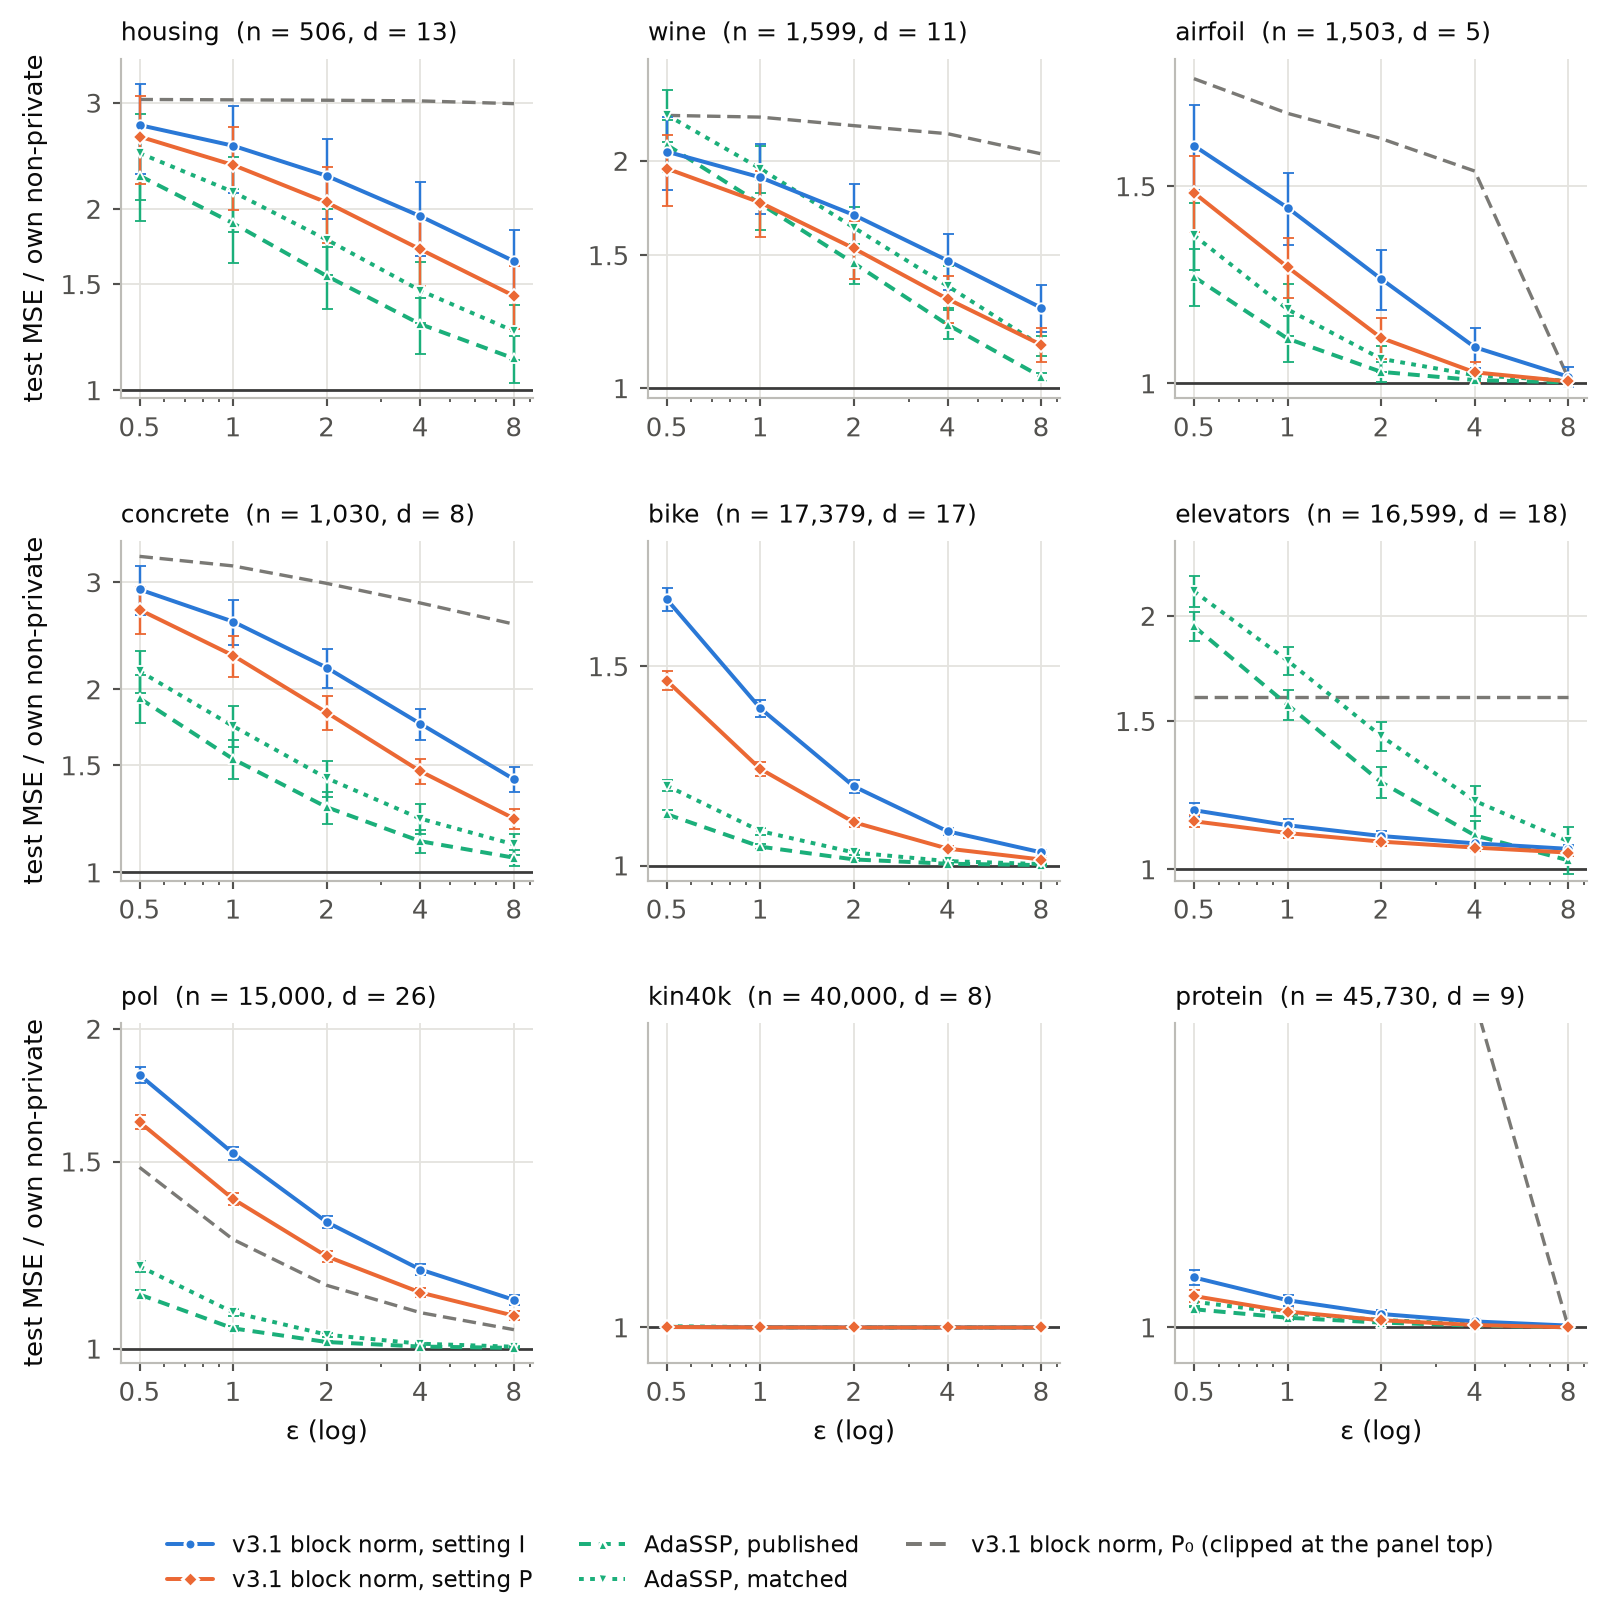
\includegraphics[width=\textwidth]{figures/adassp_mse_vs_eps_v31p2.png}
  \caption{Test MSE divided by each arm's own non-private test MSE against $\varepsilon$, $\delta = 10^{-6}$, on nine of the datasets. Blue: v3.1 with block unit norm, setting I. Orange: the same, setting P. Aqua: AdaSSP, published (dashed) and matched (dotted). Grey dashed: v3.1 with block unit norm under P$_0$, the first choice of P, clipped at the top of each panel. Points: mean over 10 folds and 50 noise draws. Error bars: 95\% CI of the mean ($t$ over folds).}
%NEW-END
%R-END R31

%R-BEGIN R32 Section 13.7 results: the two P bullets
%OLD|   \item \emph{Setting P closes the gap under joint normalization.} Arm (c) under P has a median gap of $+0.8\%$ against AdaSSP (matched) at $\varepsilon = 1$: lower test MSE on 6 datasets, higher on 11, and no significant difference on 12. At every $\varepsilon$ its median gap to (b) is between $+0.2\%$ and $+1.1\%$, and to (a) between $+7\%$ and $+9\%$. Its ridge is $1.3$ times that of AdaSSP (matched). It beats (c) under I on 20--21 datasets at every $\varepsilon$. Its gate refused $1.8\%$ of releases on average, and at most $29\%$ on any dataset and $\varepsilon$ (servo).
%OLD|   \item \emph{The implementable arm.} Under block normalization, (d) under setting I has higher test MSE than AdaSSP (published) on 20 of 29 datasets at $\varepsilon = 1$ and lower on 5; the median gap is $+25\%$ at $\varepsilon = 1$ and $+11\%$ at $\varepsilon = 8$. The previous setting, against the same AdaSSP draws, gives $+28\%$ and $+12\%$ (19 and 5 datasets at $\varepsilon = 1$ in its earlier run). Setting I has lower test MSE than the previous setting on 18--24 datasets and higher on at most 4 at every $\varepsilon$, by a median of $1$--$3\%$. On protein the gap to AdaSSP is $3.0\%$ ($0.124$ against $0.120$), and on bike it is $28\%$.
%OLD|   \item \emph{Setting P fails under block normalization.} Its gate refused $65\%$ of block-normalized releases on average over the 29 datasets and all $\varepsilon$, at least a quarter on 25 of them and all of them on elevators, gas and solar. It passes only on 3droad, kin40k and tamielectric, where the ridge is off, and on pol, where it refused at most $1\%$. A refused release outputs $\btheta = 0$, so (d) under P is worse than AdaSSP (published) by a median of $+36\%$ at $\varepsilon = 1$ and $+81\%$ at $\varepsilon = 8$, and worse than (d) under I on 16--20 datasets. Section~\ref{sec:eval:sweep} explains why block normalization makes P's gate fail.
%NEW-BEGIN
  \item \emph{Setting P narrows the gap in the implementable arm.} Under block normalization, (d) under setting P has higher test MSE than AdaSSP (published) on 20 of 29 datasets at $\varepsilon = 1$ and lower on 5, the same counts as setting I, but the median gap is $+14\%$ instead of $+25\%$. At $\varepsilon = 8$ it is higher on 15 and lower on 3 (bike, kin40k and pol), with a median gap of $+4.3\%$ ($+10.7\%$ under I). Against AdaSSP (matched) the median gap is $+6.3\%$ at $\varepsilon = 1$ and $+1.4\%$ at $\varepsilon = 8$. Setting P has lower test MSE than setting I on 18--24 datasets and higher on at most 2 at every $\varepsilon$, by a median of $3$--$7\%$. Its ridge is $0.6$ times that of I. On protein the gap to AdaSSP (published) is $2.0\%$ ($0.122$ against $0.120$), and on bike it is $13\%$. Its gate refused $0.2\%$ of releases on average over the 29 datasets and all $\varepsilon$, more than $1\%$ on at most 3 datasets at any $\varepsilon$, and at most $7.2\%$ (solar at $\varepsilon = 1$, where $\sigma_1 = 0.25\,\sigma_2$).
  \item \emph{Setting P under joint normalization.} Arm (c) under P has a median gap of $+4.9\%$ against AdaSSP (matched) at $\varepsilon = 1$ (lower test MSE on 6 datasets, higher on 18) and $+2.6\%$ at $\varepsilon = 8$ (1 and 18). Against AdaSSP (published) the gaps are $+8.8\%$ and $+7.8\%$. Its ridge is $1.6$--$1.9$ times that of AdaSSP (matched), against $2.6$--$2.9$ times under I, and it beats (c) under I on 18--21 datasets at every $\varepsilon$. Its gate refused $0.03\%$ of releases on average, and at most $2.4\%$ (servo, $\varepsilon = 8$).
  \item \emph{The first choice P$_0$ failed under block normalization.} P$_0$ ($\vartheta^\star = 0.5$, $\alpha_L = 0.5$, $f_1 = 0.2$) matched AdaSSP (matched) to within about $1\%$ under joint normalization (a median gap of $+0.2\%$ to $+1.1\%$ at every $\varepsilon$, with a ridge $1.1$--$1.4$ times AdaSSP's). Under block normalization, however, its gate refused $65\%$ of releases on average over the 29 datasets and all $\varepsilon$: at least a quarter on 25 of them, and all of them on elevators, gas and solar. A refused release outputs $\btheta = 0$, so (d) under P$_0$ was worse than AdaSSP (published) by a median of $+36\%$ at $\varepsilon = 1$ and $+81\%$ at $\varepsilon = 8$. Under joint normalization setting P is worse than P$_0$ on 18--20 datasets, by a median of $0.3$--$2.9\%$; that is the price of a gate that passes under block normalization, where P beats P$_0$ on 18--20 datasets. Section~\ref{sec:eval:sweep} explains why block normalization made P$_0$'s gate fail.
%NEW-END
%R-END R32

%R-BEGIN R33 Figure fig:sweep_v31: new file and caption
%OLD|   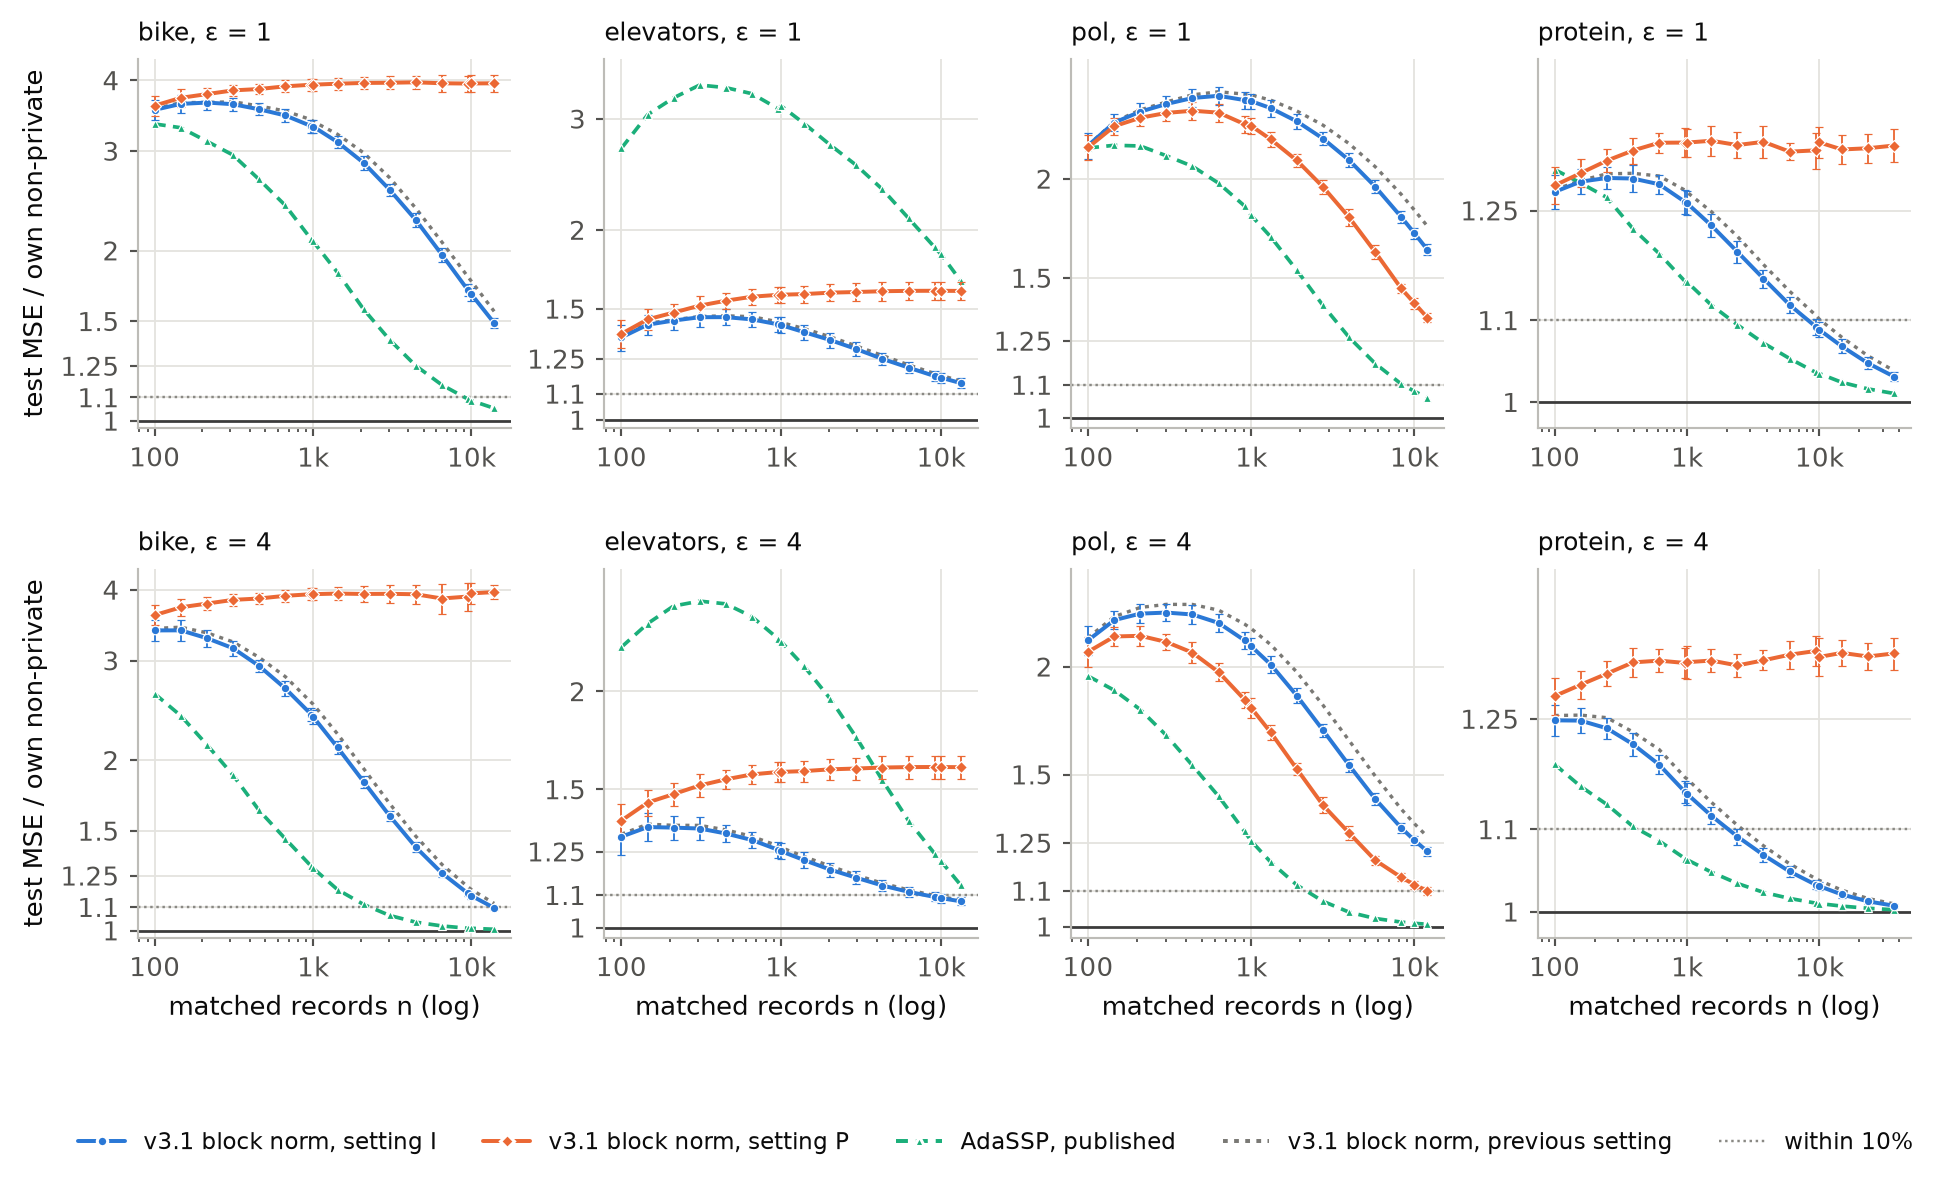
\includegraphics[width=\textwidth]{figures/sweep_n_v31s.png}
%OLD|   \caption{Test MSE divided by the arm's own non-private test MSE at the same $n$, against the number of matched records, $\delta = 10^{-9}$; top row $\varepsilon = 1$, bottom row $\varepsilon = 4$. Blue: v3.1 with block unit norm, setting I. Orange: the same, setting P. Aqua dashed: AdaSSP (published). Grey dotted: v3.1 with block unit norm at the previous setting. Error bars: 95\% CI over folds.}
%NEW-BEGIN
  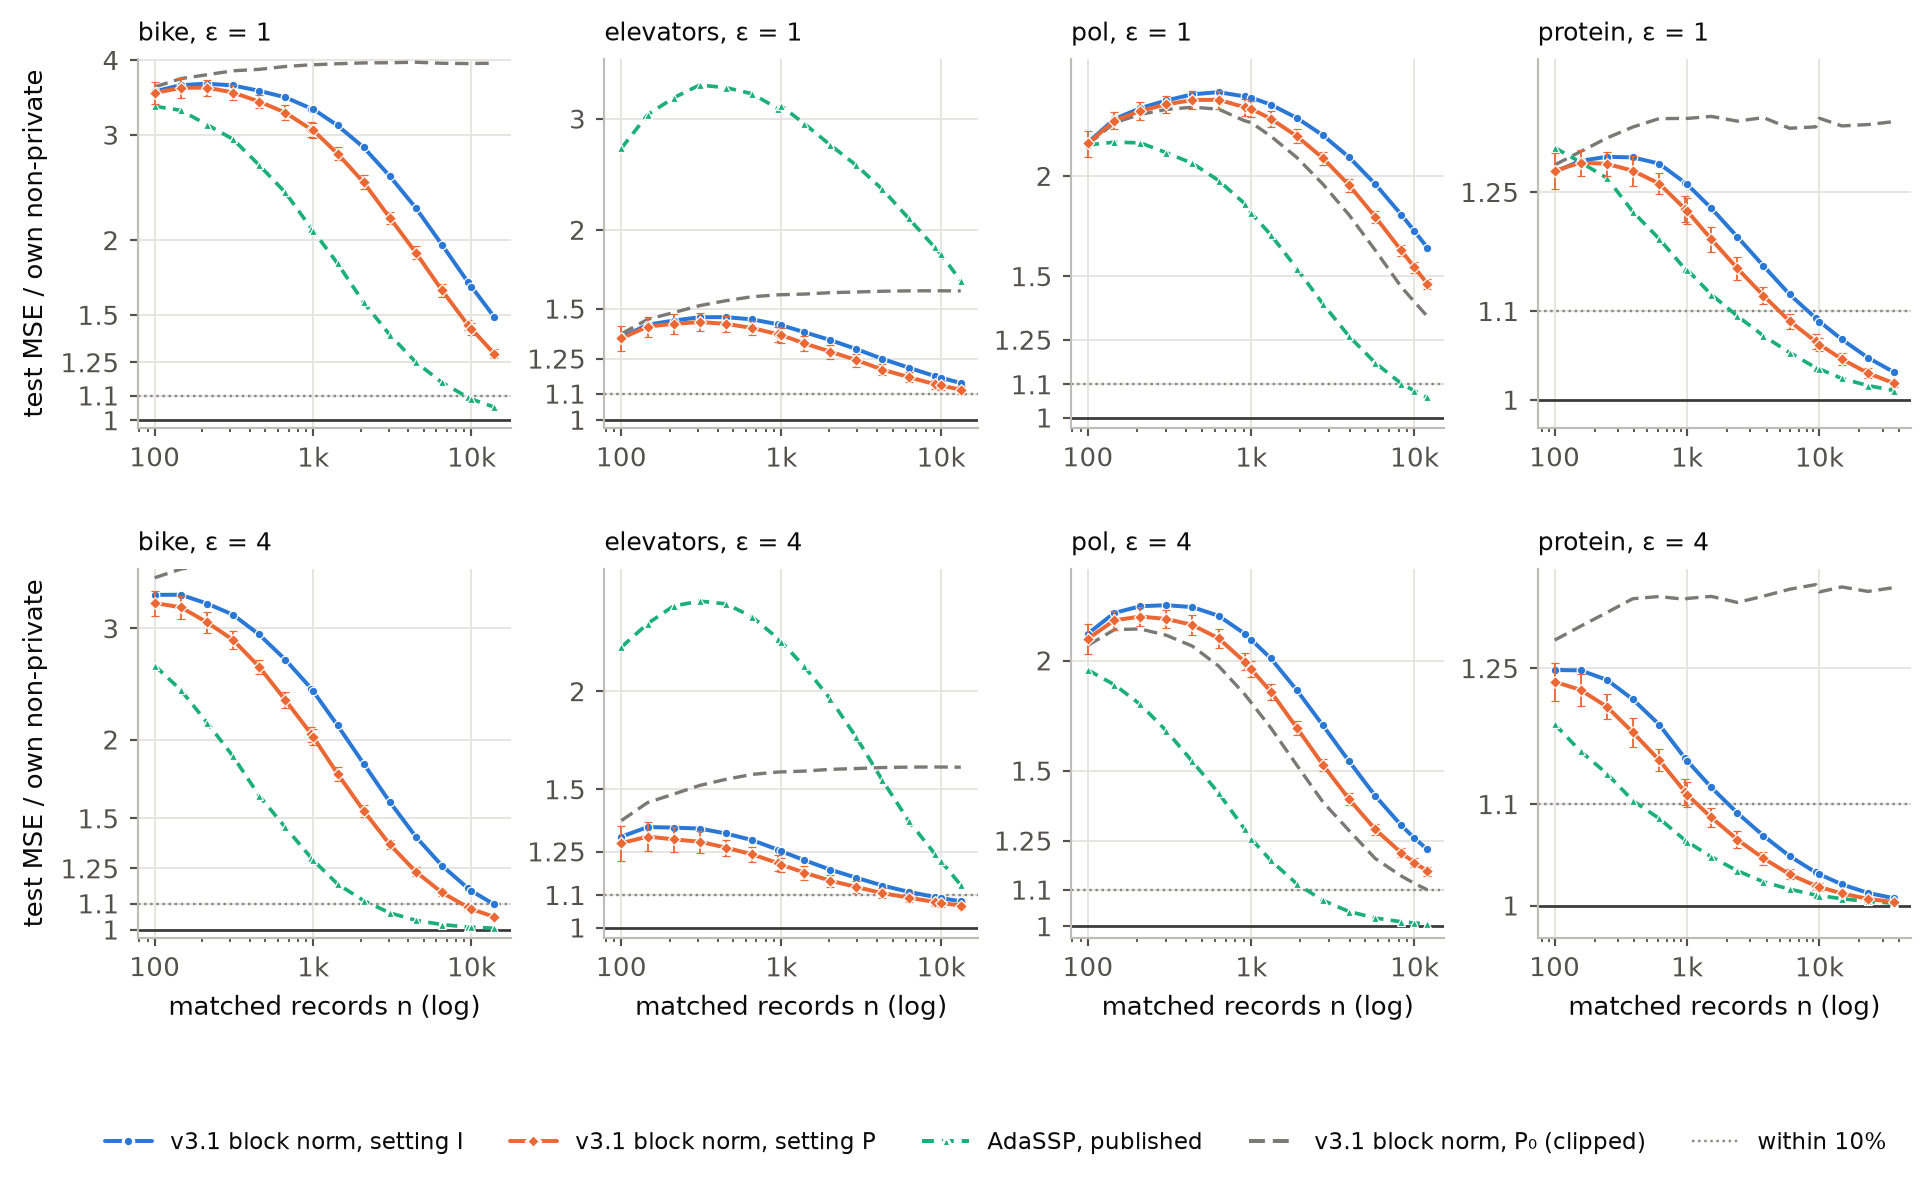
\includegraphics[width=\textwidth]{figures/sweep_n_v31p2.png}
  \caption{Test MSE divided by the arm's own non-private test MSE at the same $n$, against the number of matched records, $\delta = 10^{-9}$; top row $\varepsilon = 1$, bottom row $\varepsilon = 4$. Blue: v3.1 with block unit norm, setting I. Orange: the same, setting P. Aqua dashed: AdaSSP (published). Grey dashed: v3.1 with block unit norm under P$_0$, the first choice of P (clipped). Error bars: 95\% CI over folds (setting P).}
%NEW-END
%R-END R33

%R-BEGIN R34 Table tab:sweep_v31: caption and rows for P and P0
%OLD|   \caption{Matched records needed to come within $10\%$ of the arm's own non-private test MSE, $\delta = 10^{-9}$: v3.1 with block unit norm under settings I and P and at the previous setting, and AdaSSP (published). ``$>$'' means not reached at the sizes available.}
%OLD|   \label{tab:sweep_v31}
%OLD|   \begin{tabular}{@{}llccccc@{}}
%OLD|     \toprule
%OLD|     Dataset ($n$ available) & Arm & $\varepsilon = 0.5$ & $\varepsilon = 1$ & $\varepsilon = 2$ & $\varepsilon = 4$ & $\varepsilon = 8$ \\
%OLD|     \midrule
%OLD|     bike (13{,}903) & v3.1, I & $>$14k & $>$14k & $>$14k & 13.6k & 7.3k \\
%OLD|      & v3.1, P & $>$14k & $>$14k & $>$14k & $>$14k & $>$14k \\
%OLD|      & v3.1, previous & $>$14k & $>$14k & $>$14k & $>$14k & 8.3k \\
%OLD|      & AdaSSP & $>$14k & 9.1k & 4.5k & 2.3k & 1.2k \\
%OLD|     \midrule
%OLD|     elevators (13{,}279) & v3.1, I & $>$13k & $>$13k & $>$13k & 8.0k & 4.1k \\
%OLD|      & v3.1, P & $>$13k & $>$13k & $>$13k & $>$13k & $>$13k \\
%OLD|      & v3.1, previous & $>$13k & $>$13k & $>$13k & 8.9k & 4.7k \\
%OLD|      & AdaSSP & $>$13k & $>$13k & $>$13k & $>$13k & 8.8k \\
%OLD|     \midrule
%OLD|     pol (12{,}000) & v3.1, I & $>$12k & $>$12k & $>$12k & $>$12k & $>$12k \\
%OLD|      & v3.1, P & $>$12k & $>$12k & $>$12k & 12.0k & 6.4k \\
%OLD|      & v3.1, previous & $>$12k & $>$12k & $>$12k & $>$12k & $>$12k \\
%OLD|      & AdaSSP & $>$12k & 8.5k & 4.3k & 2.2k & 1.0k \\
%OLD|     \midrule
%OLD|     protein (36{,}584) & v3.1, I & 16k & 8.2k & 4.1k & 2.1k & 985 \\
%OLD|      & v3.1, P & $>$37k & $>$37k & $>$37k & $>$37k & 32k \\
%OLD|      & v3.1, previous & 20k & 10k & 5.2k & 2.6k & 1.3k \\
%OLD|      & AdaSSP & 4.5k & 2.2k & 992 & 427 & 166 \\
%NEW-BEGIN
  \caption{Matched records needed to come within $10\%$ of the arm's own non-private test MSE, $\delta = 10^{-9}$: v3.1 with block unit norm under settings I and P, under P$_0$ and at the previous setting, and AdaSSP (published). ``$>$'' means not reached at the sizes available.}
  \label{tab:sweep_v31}
  \begin{tabular}{@{}llccccc@{}}
    \toprule
    Dataset ($n$ available) & Arm & $\varepsilon = 0.5$ & $\varepsilon = 1$ & $\varepsilon = 2$ & $\varepsilon = 4$ & $\varepsilon = 8$ \\
    \midrule
    bike (13{,}903) & v3.1, I & $>$14k & $>$14k & $>$14k & 13.6k & 7.3k \\
     & v3.1, P & $>$14k & $>$14k & $>$14k & 8.6k & 4.5k \\
     & v3.1, P$_0$ & $>$14k & $>$14k & $>$14k & $>$14k & $>$14k \\
     & v3.1, previous & $>$14k & $>$14k & $>$14k & $>$14k & 8.3k \\
     & AdaSSP & $>$14k & 9.1k & 4.5k & 2.3k & 1.2k \\
    \midrule
    elevators (13{,}279) & v3.1, I & $>$13k & $>$13k & $>$13k & 8.0k & 4.1k \\
     & v3.1, P & $>$13k & $>$13k & 9.5k & 5.1k & 2.5k \\
     & v3.1, P$_0$ & $>$13k & $>$13k & $>$13k & $>$13k & $>$13k \\
     & v3.1, previous & $>$13k & $>$13k & $>$13k & 8.9k & 4.7k \\
     & AdaSSP & $>$13k & $>$13k & $>$13k & $>$13k & 8.8k \\
    \midrule
    pol (12{,}000) & v3.1, I & $>$12k & $>$12k & $>$12k & $>$12k & $>$12k \\
     & v3.1, P & $>$12k & $>$12k & $>$12k & $>$12k & 10.5k \\
     & v3.1, P$_0$ & $>$12k & $>$12k & $>$12k & 12.0k & 6.4k \\
     & v3.1, previous & $>$12k & $>$12k & $>$12k & $>$12k & $>$12k \\
     & AdaSSP & $>$12k & 8.5k & 4.3k & 2.2k & 1.0k \\
    \midrule
    protein (36{,}584) & v3.1, I & 16k & 8.2k & 4.1k & 2.1k & 985 \\
     & v3.1, P & 10k & 5.0k & 2.5k & 1.2k & 599 \\
     & v3.1, P$_0$ & $>$37k & $>$37k & $>$37k & $>$37k & 32k \\
     & v3.1, previous & 20k & 10k & 5.2k & 2.6k & 1.3k \\
     & AdaSSP & 4.5k & 2.2k & 992 & 427 & 166 \\
%NEW-END
%R-END R34

%R-BEGIN R35 Section 13.8: P and P0 bullets
%OLD|   \item \emph{Setting P is refused by the gate on three of the four datasets.} While the ridge is on, the gate refused $96$--$100\%$ of P's releases on bike, $100\%$ on elevators and $82$--$97\%$ on protein, at every $n$ and $\varepsilon$. A refused release outputs $\btheta = 0$ and still spends the budget, so P's test MSE stays near that of predicting the mean: at the largest $n$ it is $3.9$, $1.6$ and $1.34$ times non-private. P reaches $10\%$ on protein only at $\varepsilon = 8$, where its ridge switches off ($32$k). On pol the gate refused at most $2\%$ of P's releases, and there P beats I: within $10\%$ at $12.0$k ($\varepsilon = 4$) and $6.4$k ($\varepsilon = 8$), and $1.34$ and $1.10$ times non-private at $12$k for $\varepsilon = 1$ and $4$.
%OLD|   \item \emph{Why P fails here.} With $\vartheta^\star = 0.5$ the gate passes only if $r_1$ exceeds $\sigma_2\sqrt p$ by more than the extra downward shift that the stage-2 noise causes in $\lambda_{\min}$ (Section~\ref{sec:stats:stage2}). On the synthetic population, where $\Delta_G \approx 0.9\Delta$, P has $\sigma_1 = 1.79\,\sigma_2$ and $r_1 = 8.9\,\sigma_2$, far above $\sigma_2\sqrt{11} = 3.3\,\sigma_2$. Block normalization bounds $\bx$ tightly but leaves $B_y$ as large as before, so $\Delta_G/\Delta \approx 0.34$ on protein. Then $\sigma_1 \approx 0.67\,\sigma_2$ and $r_1 = q_{0.5}\sigma_1 \approx 4.53 \times 0.67\,\sigma_2 \approx 3.1\,\sigma_2$ ($p = 10$), below $\sigma_2\sqrt{10} = 3.2\,\sigma_2$ even before the stage-2 noise, the larger of the two, lowers $\lambda_{\min}$ further. The selection population never entered this regime, so the pre-registered rule could not see it.
%NEW-BEGIN
  \item \emph{Setting P.} Its gate refused at most $1\%$ of releases at every $n$ and $\varepsilon$ on all four datasets: at most $0.3\%$ on bike, $1.0\%$ on elevators, and none on pol and protein. P comes within $10\%$ sooner than setting I wherever either does. On protein it needs $10$k, $5.0$k, $2.5$k, $1.2$k and $599$ matched records for $\varepsilon = 0.5$ to $8$, $1.6$--$1.7$ times fewer than I. On bike it needs $8.6$k and $4.5$k for $\varepsilon = 4$ and $8$ (I: $13.6$k and $7.3$k). On elevators it needs $9.5$k, $5.1$k and $2.5$k for $\varepsilon = 2$, $4$ and $8$, where I needed $8.0$k and $4.1$k for $\varepsilon = 4$ and $8$ only. On pol it gets there at $\varepsilon = 8$ only ($10.5$k). AdaSSP still needs $2.2$--$3.6$ times fewer records than P on protein. At the largest $n$ and $\varepsilon = 1$ the median stage-1 ridge under P is $600$ on protein and $1{,}204$ on bike, against $1{,}056$ and $1{,}936$ under I.
  \item \emph{Why the first choice P$_0$ failed.} While the ridge was on, the gate refused $96$--$100\%$ of P$_0$'s releases on bike, $100\%$ on elevators and $82$--$97\%$ on protein, at every $n$ and $\varepsilon$. A refused release outputs $\btheta = 0$ and still spends the budget, so P$_0$'s test MSE stayed near that of predicting the mean: at the largest $n$ it was $3.9$, $1.6$ and $1.34$ times non-private. With $\vartheta^\star = 0.5$ the gate passes only if $r_1$ exceeds $\sigma_2\sqrt p$ by more than the extra downward shift that the stage-2 noise causes in $\lambda_{\min}$ (Section~\ref{sec:stats:stage2}). On the standardized synthetic population, where $\Delta_G \approx 0.9\Delta$, P$_0$ had $\sigma_1 = 1.79\,\sigma_2$ and $r_1 = 8.9\,\sigma_2$, far above $\sigma_2\sqrt{11} = 3.3\,\sigma_2$. Block normalization bounds $\bx$ tightly but leaves $B_y$ as large as before, so $\Delta_G/\Delta \approx 0.34$ on protein. Then $\sigma_1 \approx 0.67\,\sigma_2$ and $r_1 = q_{0.5}\sigma_1 \approx 4.53 \times 0.67\,\sigma_2 \approx 3.1\,\sigma_2$ ($p = 10$), below $\sigma_2\sqrt{10} = 3.2\,\sigma_2$ even before the stage-2 noise, the larger of the two, lowers $\lambda_{\min}$ further. P$_0$'s selection population never entered this regime. Setting P's selection included a block-normalized population with $\sigma_1 = 0.46\,\sigma_2$, and with $\vartheta^\star = 1.5$ its gate does not depend on $r_1$ to pass. On pol, where $\sigma_1 = 0.83\,\sigma_2$ under P, the gate refused at most $2\%$ of P$_0$'s releases, and there P$_0$ remains the best v3.1 arm: within $10\%$ at $12.0$k ($\varepsilon = 4$) and $6.4$k ($\varepsilon = 8$).
%NEW-END
%R-END R35

%R-BEGIN R36 Check item on P's selection population
%OLD| \tocheck{Setting P was chosen on a synthetic population with Delta-G about 0.9 Delta, where its gate never refuses; on block-normalized real data (Delta-G about 0.34 Delta on protein) the gate refuses 82-100 percent of its releases on bike, elevators and protein. A prediction setting needs a selection rule that covers this regime, for example a selection population with block-normalized features, or theta-star at least 1, and a new pre-registered choice validated on fresh data.}
%NEW-BEGIN
\tocheck{Setting P was re-chosen on a standardized and a block-normalized synthetic population after P-0 failed on block-normalized real data, and its gate refused at most 1 percent of releases on the four sweep datasets. On the 29 benchmark datasets it refused up to 7 percent on solar (sigma-1 = 0.25 sigma-2, below the selection's range); check P on further datasets with heavy-tailed y before relying on it there.}
%NEW-END
%R-END R36

%R-BEGIN R37 Section 13.9: sigma_2 under P at unit bounds
%OLD| $\sigma_2 = 16.5$ at setting I, $16.0$ at P and $15.1$ at the previous setting
%NEW-BEGIN
$\sigma_2 = 16.5$ at settings I and P (both $f_1 = 0.25$) and $15.1$ at the previous setting
%NEW-END
%R-END R37

%R-BEGIN R38 Section 13.9: the setting-P bullet
%OLD|   \item \emph{Setting P gives up the interval guarantee.} With joint normalization its ridge is $1.3$ times that of AdaSSP (matched), and it matches that arm to within about $1\%$ in median test MSE. With block normalization, the preprocessing a vertical deployment can use, its gate refuses most releases and it is the worst v3.1 arm. The gate is part of the protocol: with $\vartheta^\star < 1$ it passes only when the stage-1 noise is not much smaller than the stage-2 noise ($\sigma_1 = 1.34\,\sigma_2$ for unit bounds, about $0.67\,\sigma_2$ for block-normalized protein), and block normalization makes $\Delta_G$ about a third of $\Delta$. A prediction setting that works under block normalization has not yet been chosen or evaluated.
%NEW-BEGIN
  \item \emph{Setting P gives up the interval guarantee.} It holds the validity ratio at about $3.5$ instead of $5$ ($2.0$ on the block-normalized population), its ridge is about $0.6$ times that of setting I, and its gate still passes: it was chosen under a bound on refusals on standardized and block-normalized synthetic data, and it refused $0.2\%$ of block-normalized releases on average over the 29 datasets. With block normalization, the preprocessing a vertical deployment can use, it is the best v3.1 arm. It is better than setting I on 18--24 datasets at every $\varepsilon$, and the median gap to AdaSSP (published) falls from $+25\%$ to $+14\%$ at $\varepsilon = 1$ and from $+11\%$ to $+4\%$ at $\varepsilon = 8$. It is still worse than AdaSSP on 20 of 29 datasets at $\varepsilon = 1$. Under joint normalization its ridge is $1.8$ times that of AdaSSP (matched). The first choice P$_0$ ($\vartheta^\star = 0.5$) came within about $1\%$ of AdaSSP (matched) there, with a ridge $1.3$ times AdaSSP's, but was refused on most block-normalized releases. With $\vartheta^\star < 1$ the gate passes only when the stage-1 noise is not much smaller than the stage-2 noise ($\sigma_1 = 1.34\,\sigma_2$ for unit bounds, about $0.67\,\sigma_2$ for block-normalized protein), and block normalization makes $\Delta_G$ about a third of $\Delta$.
%NEW-END
%R-END R38

%R-BEGIN R39 Summary: the setting-P sentences
%OLD| Setting P gives up the intervals for a smaller ridge. It predicts best on the synthetic population, but on block-normalized real data its gate refuses most releases, so a prediction setting remains open.
%NEW-BEGIN
Setting P gives up the intervals for a smaller ridge. It was chosen subject to a bound on gate refusals, after a first choice failed on block-normalized real data. With block normalization it beats setting I on 18--24 of 29 datasets at every $\varepsilon$ and nearly halves the median gap to AdaSSP at $\varepsilon = 1$ ($+14\%$ against $+25\%$), but AdaSSP on the joined table still predicts better on 20 of them.
%NEW-END
%R-END R39
